\documentclass[compress,t]{beamer}

%%%%%%%%%%%%%%%%%%%%%%%%%%%%%%%%%%%%%%%%%%%%%%%%%%
% Optional packages, used to show off certain tricks
\usepackage{./beamerthemeOSU}

% If you don't like the section navigation things at the top of your page, you can
% uncomment this command, and they all go away.
%\setbeamertemplate{headline}{}

%%%%%%%%%%%%%%%%%%%%%%%%%%%%%%%%%%%%%%%%%%%%%%%%%%

%\mode<presentation>{}

\newcommand{\SN}{$S_N$}
\newcommand{\RZ}{$R$-$Z$}
\newcommand{\XY}{$X$-$Y$}
%\usepackage{bm}
\renewcommand{\vec}[1]{\boldsymbol{#1}} %vector is bold italic
\newcommand{\vd}{\boldsymbol{\cdot}} % slightly bold vector dot
\newcommand{\grad}{\vec{\nabla}} % gradient
\newcommand{\ud}{\mathop{}\!\mathrm{d}} % upright derivative symbol

\usepackage{tikz}
\usepackage{tikz-3dplot}
\usetikzlibrary{patterns, shapes.geometric, arrows,calc}
\usepackage{pgfplots}
\usetikzlibrary{patterns}
\usepackage{mathtools}
\DeclarePairedDelimiterX{\norm}[1]{\lVert}{\rVert}{#1}

\usepackage{hyperref}
\usepackage[makeroom]{cancel}
\usepackage{soul} % to use \ul for underlines that line wrap
\usepackage{subcaption} % subfigure

\usepackage{appendixnumberbeamer} % restart page numbering for \appendix slides

\title{Discrete Ordinates Radiation Transport using Higher-Order Finite Element Spatial Discretizations on Meshes with Curved Surfaces}

\author[1]{Douglas N. Woods}

\date{4 June 2018}

\subtitle{Dissertation Defense}
% There is a default document number to remind you to get your talk approved.
%\docnumber{LLNL-PRES-XXXXXX}

%%%%%%%%%%%%%%%%%%%%%%%%%%%%%%%%%%%%%%%%%%%
\begin{document}

\setlength{\abovedisplayskip}{5pt}
\setlength{\belowdisplayskip}{5pt}

%%%%%%%%%%%%%%%%%%%%%%%%%%%%%%%%%%%%%%%%%%%
%  All this typeout stuff simply gets printed to the screen as the document
% is compiled.  It helps get stuff working
\typeout{*******************************************************************}
\typeout{titlepage}
\begin{frame}[label=title,plain] %need the plain to make the title slide different than the rest of the slides!
%\maketitle
\titlepage
\end{frame}

%%%%%%%%%%%%%%%%%%%%%%%%%%%%%%%%%%%%%%%
\section{Introduction}
\subsection{}

\begin{frame}
\frametitle{Outline}

\begin{columns}[T]

\column{\textwidth}
\begin{itemize}
\item{Introduction}
\item{Objectives}
\item{Methods}
\item{MIP DSA}
\begin{itemize}
\item{Implementation}
\item{Numerical Results}
\end{itemize}
\item{\RZ\ Geometry}
\begin{itemize}
\item{Implementation}
\item{Numerical Results}
\end{itemize}
\item{Conclusions}
\end{itemize}

\column{0.0\textwidth}
\begin{figure}[!h]
\flushright
%\includegraphics[scale=0.15]{../../../Research/graphics/nifShot.jpg}
\vspace{-8pt}
%\flushright\tiny{\url{https://lasers.llnl.gov/content/assets/images/media/photo-gallery/large/nif-1209-18059.jpg}}
\end{figure}

\end{columns}

\end{frame}

%%%%%%%%%%%%%%%%%%%%%%%%%%%%%%%%%%%%%%%
\section{Introduction}
\subsection{}

\setbeamercovered{invisible}
\begin{frame}
\frametitle{Introduction}
\framesubtitle{Radiation-hydrodynamics}

\begin{columns}[T]

\column{0.5\textwidth}
\begin{itemize}
\item{High energy density physics}
\begin{itemize}
\item{astrophysics}
\item{inertial confinement fusion}
\end{itemize}
\onslide<2->{
\item{Blackbody radiation can influence the energy, temperature, momentum, pressure of the fluid}}
\onslide<3->{
\item{Radiation-hydrodynamics to study these problems}}
\onslide<4->{
\item{Can study radiation transport and hydrodynamics separately}}
\end{itemize}

\column{0.5\textwidth}
\begin{figure}[!h]
\flushright
\includegraphics[scale=0.15]{../../../Research/graphics/nifShot.jpg}
\vspace{-8pt}
\flushright\tiny{\url{https://lasers.llnl.gov/content/assets/images/media/photo-gallery/large/nif-1209-18059.jpg}}
\end{figure}

\end{columns}

\end{frame}

%%%%%%%%%%%%%%%%%%%%%%%%%%%%%%%%%%%%%%%
\section{Introduction}
\subsection{}

\setbeamercovered{invisible}
\begin{frame}
\frametitle{Introduction}
\framesubtitle{BLAST --- LLNL ALE hydrodynamics code}

\begin{columns}[T]
\column{0.45\textwidth}
\begin{centering}
\includegraphics[width=\textwidth,trim={0 0 0 0},clip]{../../../Research/graphics/triple-point_BLAST_q8q7.png}
\end{centering}
\tiny{https://computation.llnl.gov/project/blast/}

\column{0.55\textwidth}
\vspace{10pt}
\footnotesize{\par multi-material shock hydrodynamics problem solved with BLAST: $8^\text{th}$-order kinematics, $7^\text{th}$-order thermodynamics}
\end{columns}

\begin{itemize}
\item{High-order (HO) finite element spatial discretization}
\onslide<2->{
\item{Meshes with curved surfaces}
\begin{itemize}
\item{Straight-edged meshes restrict the accuracy of the compressible Euler equations}
\item{ ``Essential for higher-order accuracy''}
\end{itemize}}
\onslide<3->{
\item{More accurately model:}
\begin{itemize}
\item{Fluid flow geometry in Lagrangian framework with curved meshes}
\item{Can model a shock front within a single zone - higher resolution}
\item{Radial flow symmetry}
\end{itemize}}
\end{itemize}

\end{frame}

%%%%%%%%%%%%%%%%%%%%%%%%%%%%%%%%%%%%%%%
% Empty subsection required to get the dots to show up in navigation bar
\subsection{}
%%%
\begin{frame}
\frametitle{Introduction}
\framesubtitle{High-order radiation transport}

\begin{itemize}
\item{HO $(p \geq 2)$ \SN\ transport FEM research is relatively new}
\begin{itemize}
\item{FEM approximates the solution to be a polynomial expansion}
\item{Low-order (LO) $(p=1)$ methods are less computationally expensive}
\item{Expected spatial convergence of $O(p+1)$ have been shown}
\item{HO DFEMs are accurate in the diffusion limit}
\item{Some HO DFEM research in 1-D thermal radiation transport}
\end{itemize}
\onslide<2->{
\item{\RZ\ geometry has only been explored using LO finite elements}
\begin{itemize}
\item{$2^\text{nd}$-order spatial convergence for linear methods (BLD, PWLD, etc.)}
\item{Accurate in the diffusion limit}
\end{itemize}}
\onslide<3->{
\item{Structured/unstructured quadrilateral and triangular meshes}
\begin{itemize}
\item{Some research for meshes with curved surfaces}
\item{Do not degrade $O(p+1)$ spatial convergence rate}
\end{itemize}}
%\item{Source iteration acceleration using MIP DSA}
\end{itemize}

\end{frame}

%%%%%%%%%%%%%%%%%%%%%%%%%%%%%%%%%%%%%%%
% Empty subsection required to get the dots to show up in navigation bar
\subsection{}
%%%
\begin{frame}
\frametitle{Objectives}

\begin{itemize}
\item{Use MFEM, a general finite element library (\url{mfem.org}):}
\end{itemize}
\begin{enumerate}
\item{Modified interior penalty (MIP) diffusion synthetic acceleration (DSA)}
\begin{itemize}
\item{Implement MIP DSA equations using homogeneous \ul{Robin} (i.e. vacuum) boundary conditions}
\item{Examine and compare spectral radii to MIP DSA using homogeneous \ul{Dirichlet} boundary conditions}
\end{itemize}
\onslide<2->{
\item{\RZ\ geometry}
\begin{itemize}
\item{Numerically solve HO \SN\ transport equation on meshes with curved surfaces}
\item{Perform spatial convergence studies}
\item{Preserve 1-D spherical symmetry}
\end{itemize}}
\end{enumerate}

\end{frame}

%%%%%%%%%%%%%%%%%%%%%%%%%%%%%%%%%%%%%%%
% Empty subsection required to get the dots to show up in navigation bar
\subsection{}
\begin{frame}
\frametitle{Methods}
\framesubtitle{HO DGFEM spatial discretization}

\begin{itemize}
\item{Steady-state, monoenergetic radiation transport equation}
{\small
\begin{flalign*}
\vec{\Omega}_m \vd \grad \psi_m + \sigma_t \psi_m & = \frac{1}{4 \pi} \sigma_s \phi + \frac{1}{4 \pi} S_0 \\
\phi & = \sum_m w_m \psi_m
\end{flalign*}}
\onslide<2->{
\item{Standard discontinuous Galerkin finite element method (DGFEM) spatial discretization}
{\small
\begin{flalign*}
\left(\vec{\Omega}_m \vd \grad \psi_m,v_i \right)_{\mathcal{D}_k} + \left(\sigma_t \psi_m, v_i \right)_{\mathcal{D}_k} & = \frac{1}{4 \pi} \left(\sigma_s \phi, v_i \right)_{\mathcal{D}_k} + \frac{1}{4 \pi} \left(S_0,v_i \right)_{\mathcal{D}_k} \\
\psi_m & \approx \sum_j b_j(\vec{x}) \psi_{j,m}
\end{flalign*}}}
\end{itemize}

\end{frame}

%%%%%%%%%%%%%%%%%%%%%%%%%%%%%%%%%%%%%%%
% Empty subsection required to get the dots to show up in navigation bar
\subsection{}
\begin{frame}
\frametitle{Methods}
\framesubtitle{$2^\text{nd}$-order basis functions allow for more complex solution shapes on each element}

\begin{columns}[T]

\column{0.4\textwidth}
\centering
\includegraphics[width=\textwidth]{../../../Research/graphics/BasisE2Edge}

\includegraphics[width=\textwidth]{../../../Research/graphics/BasisE2Corner}


\column{0.4\textwidth}
\centering
\includegraphics[width=\textwidth]{../../../Research/graphics/BasisE2mid}

\begin{flalign*}
b_j(x,y) & = c_1 x^2 y^2 + c_2 x^2 y + c_3 x^2 \\
& + c_4 x y^2 + c_5 x y + c_6 x \\
& + c_7 y^2 + c_8 y + c_9
\end{flalign*}

\end{columns}

\end{frame}

%%%%%%%%%%%%%%%%%%%%%%%%%%%%%%%%%%%%%%%
% Empty subsection required to get the dots to show up in navigation bar
\subsection{}
\begin{frame}
\frametitle{Methods}
\framesubtitle{HO mapping allows for meshes with curved surfaces}

\begin{figure}[!htb]
\centering
\begin{subfigure}{0.4\textwidth}
\footnotesize
\begin{tikzpicture}
\hspace{-10pt}
\begin{axis}[
	axis lines=left,
	width=\textwidth,
	height=\textwidth,
    xmin=0.9, xmax=2.5,
    ymin=0.8, ymax=2.5,
    xlabel={$x$},
    ylabel={$y$},
    ]
    \addplot[only marks, mark=*, mark size=1, color=red, mark options={solid, fill=red}] table [x index=0, y index=1]{../../../Research/graphics/MeshTransform.dat};
    \addplot[only marks, mark=*, mark size=3, color=black, mark options={solid, fill=black}] table [x index=0, y index=1]{../../../Research/graphics/MeshTransNodes.dat};
\end{axis}
\end{tikzpicture}
\centering
\footnotesize{Physical element}
\end{subfigure}%
\begin{minipage}{0.12\textwidth}
\centering
\vspace{-30pt}
\hspace{-30pt}
{\large$\mapsto$}
\end{minipage}
\begin{subfigure}{0.4\textwidth}
\footnotesize
\begin{tikzpicture}
\hspace{-20pt}
\begin{axis}[
	axis lines=left,
	width=\textwidth,
	height=\textwidth,
    xmin=0, xmax=1,
    ymin=0, ymax=1,
    xlabel={$\rho$},
    ylabel={$\kappa$},
    ]
    \addplot[only marks, mark=*, mark size=1, color=blue, mark options={solid, fill=blue}] table [x index=0, y index=1]{../../../Research/graphics/MeshReference.dat};
    \addplot[only marks, mark=*, mark size=3, color=black, mark options={solid, fill=black}] table [x index=0, y index=1]{../../../Research/graphics/MeshNodes.dat};
\end{axis}
\end{tikzpicture}
\centering
\footnotesize{Reference element}
\end{subfigure}
\end{figure}

%\begin{itemize}
%\item{Apply $\det(J)$ to the numerical integrations}
%\vspace{-10pt}
%\small
%\begin{flalign*}
%\left(a(x,y),b(x,y) \right)_{\mathcal{D}_k} & \approx \sum_{i,j}^\zeta w_i\ w_j\ a(\rho_{i},\kappa_{j})\ b(\rho_{i},\kappa_{j})\ |J_k|
%\end{flalign*}
%\end{itemize}

\end{frame}

%%%%%%%%%%%%%%%%%%%%%%%%%%%%%%%%%%%%%%%
\subsection{}

\begin{frame}
\frametitle{Methods}
\framesubtitle{HO mesh transformation example}

\begin{figure}[!htb]
\centering
\begin{subfigure}{0.45\textwidth}
\centering
\includegraphics[width=\textwidth,trim={2.5cm 2cm 1cm 1cm},clip]{../../../Research/graphics/mesh/MMSr0g0}

{\small Orthogonal mesh}
\end{subfigure}%
\hspace{0.05\textwidth}
\begin{subfigure}{0.45\textwidth}
\centering
\includegraphics[width=\textwidth,trim={2.5cm 2cm 1cm 1cm},clip]{../../../Research/graphics/mesh/MMSr0g3}

{\small $3^\text{rd}$-order mesh}
\end{subfigure}
\end{figure}

\end{frame}

%%%%%%%%%%%%%%%%%%%%%%%%%%%%%%%%%%%%%%%
% Empty subsection required to get the dots to show up in navigation bar
\subsection{}
%%%
\begin{frame}
\frametitle{Methods}
\framesubtitle{Create DGFEM matrices using MFEM, solve using a direct solver}

\begin{itemize}
\item{MFEM generates local matrices and vectors for a variety of operators, assembles them into global linear algebra system}
\begin{itemize}
\item{High-order finite elements}
\item{Create and transform meshes with curved surfaces}
%\item{No spatial sweep to avoid handling cycles}
\end{itemize}
\onslide<2->{
\item{Solve linear system directly with UMFPack ({\scriptsize \url{http://faculty.cse.tamu.edu/davis/suitesparse.html}})}
\item{Visualize solutions with VisIt ({\scriptsize \url{https://wci.llnl.gov/simulation/computer-codes/visit}})}}
\end{itemize}

\end{frame}

%%%%%%%%%%%%%%%%%%%%%%%%%%%%%%%%%%%%%%%
%%%%%%%%%%%%%%%%%%%%%%%%%%%%%%%%%%%%%%%
%%%%%%%%%%%%%%%%%%%%%%%%%%%%%%%%%%%%%%%
%%%%%%%%%%%%%%%%%%%%%%%%%%%%%%%%%%%%%%%
\section{Diffusion Synthetic Acceleration}
\subsection{}

\setbeamercovered{invisible}
\begin{frame}
\frametitle{Diffusion Synthetic Acceleration}
\framesubtitle{Source iteration acceleration}

\begin{itemize}
\item{Source iteration to solve radiation transport equation}
\begin{itemize}
\item{Iterate on scalar flux until scattering source converges}
\item{Can converge arbitrarily slowly with increased scattering}
\end{itemize}
\begin{flalign*}
\vec{\Omega} \vd \grad \psi_m^{(\ell+1)} + \sigma_t \psi_m^{(\ell+1)} & = \frac{1}{4 \pi} \sigma_s {\color{blue}\phi^{(\ell)}} + \frac{1}{4 \pi} S_0
\end{flalign*}
\begin{flalign*}
{\color{blue}\phi^{(\ell+1)}} & = \sum_{m} w_m \psi_m^{(\ell+1)}
\end{flalign*}
%\item<2->{Optical thickness}
%\begin{itemize}
%\item{Material cross section can increase/reduce transport through material}
%\item{Optically thin - few mean-free-paths (mfp) thick}
%\item{Optically thick - many mfp thick}
%\item{Refine mesh or use diffusion equation}
%\end{itemize}
\onslide<2->
\item{Source iteration acceleration}
\begin{itemize}
\item{Solve diffusion equation to make a small ``correction'' to the radiation transport solution}
\end{itemize}
\end{itemize}

\end{frame}

%%%%%%%%%%%%%%%%%%%%%%%%%%%%%%%%%%%%%%%
\section{Methods}
\subsection{}

\setbeamercovered{invisible}
\begin{frame}
\frametitle{Diffusion Synthetic Acceleration}
\framesubtitle{DSA algorithm}

\begin{itemize}
\item{Diffusion synthetic acceleration (DSA) algorithm}
\begin{flalign*}
\vec{\Omega} \vd \grad \psi_m^{(\ell+1/2)} + \sigma_t\ \psi_m^{(\ell+1/2)} & = \frac{1}{4 \pi} \sigma_s\ \phi^{(\ell)} + \frac{1}{4 \pi} S_0 \\
{\color<3>{blue}\phi^{(\ell+1/2)}} & = \sum_{m=1}^M w_m\ \psi_m ^{(\ell+1/2)} \\
\onslide<2->{
- \grad \vd D\ \grad \varphi^{(\ell+1/2)} + \sigma_a\ \varphi^{(\ell+1/2)} & = \sigma_s \left(\phi^{(\ell+1/2)} - \phi^{(\ell)} \right)} \\
\onslide<3->{
\phi^{(\ell+1)} & = {\color{blue}\phi^{(\ell+1/2)}} + \varphi^{(\ell+1/2)}}
\end{flalign*}
\end{itemize}

\end{frame}

%%%%%%%%%%%%%%%%%%%%%%%%%%%%%%%%%%%%%%%
\section{MIP DSA}
\subsection{}

\begin{frame}
\frametitle{Modified Interior Penalty DSA}
\framesubtitle{Implemented with homogeneous \ul{Dirichlet} boundary conditions}

\begin{itemize}
\item{Wang and Ragusa (2010) derived modified interior penalty (MIP) DSA with homogeneous Dirichlet boundary conditions}
\onslide<2->
\item{Bilinear form:}
\begin{multline*}
b_{MIP,D} \left(\varphi, v \right) = \left(\sigma_a\ \varphi, v \right)_\mathcal{D} + \left(D\ \grad \varphi, \grad v \right)_\mathcal{D} \\
+ \left({\color{blue}\kappa_e}\ \llbracket \varphi \rrbracket, \llbracket v \rrbracket \right)_{\partial \mathcal{D}^i}
+ \left(\llbracket \varphi \rrbracket, \left\{\!\left\{D\ \partial_n v \right\}\!\right\} \right)_{\partial \mathcal{D}^i} + \left(\left\{\!\left\{D\ \partial_n\ \varphi \right\}\!\right\}, \llbracket v \rrbracket \right)_{\partial \mathcal{D}^i} \\
+ \left({\color{blue}\kappa_e}\ \varphi, v \right)_{\partial \mathcal{D}^d}
- \frac{1}{2} \left(\varphi, D\ \partial_n v \right)_{\partial \mathcal{D}^d} - \frac{1}{2} \left(D\ \partial_n\ \varphi, v \right)_{\partial \mathcal{D}^d}
\end{multline*}
\onslide<3->
\item{Linear form:}
\begin{flalign*}
\ell_{MIP} \left( v \right) = \left(\sigma_s \left[\phi^{(\ell+1/2)} - \phi^{(\ell)} \right], v \right)_\mathcal{D}
\end{flalign*}
\end{itemize}

\end{frame}

%%%%%%%%%%%%%%%%%%%%%%%%%%%%%%%%%%%%%%%
\section{Methods}
\subsection{}

%\setbeamercovered{transparent}

\begin{frame}
\frametitle{Modified Interior Penalty DSA}
\framesubtitle{Stabilization parameter is a function of an arbitrary coefficient}

\begin{itemize}
\item{``Switch'' within the stabilization parameter between diffusion conforming form (DCF) and interior penalty (IP) method}
\begin{flalign*}
\color<1>{blue}\kappa_e & = \max \left({\color<2>{blue}\kappa_e^{IP}}, \frac{1}{4} \right) \\
\onslide<2->{{\color<2>{blue}\kappa_e^{IP}} & = \begin{cases} \frac{{\color<3>{blue}f \left( p^+ \right)}}{2} \frac{D^+}{h^+_{\bot}} + \frac{{\color<3>{blue}f \left( p^- \right)}}{2} \frac{D^-}{h^-_\bot}, & \text{on interior edges} \\
{\color<3>{blue}f \left( p \right)} \frac{D}{h_{\bot}}, & \text{on boundary edges} \end{cases} \\}
\onslide<3->{{\color<3>{blue}f \left( p \right)} & = {\color<4>{blue}C}\ p \left( p +1 \right)}
\end{flalign*}
\onslide<4->\item{{\color{blue}$C$} is an arbitrary constant $(\text{i.e. }2,4,6)$}
\end{itemize}

\end{frame}

%%%%%%%%%%%%%%%%%%%%%%%%%%%%%%%%%%%%%%%
\section{Methods}
\subsection{}

\begin{frame}
\frametitle{Modified Interior Penalty DSA}
\framesubtitle{Implemented with homogeneous \ul{Robin} boundary conditions}

\begin{itemize}
\item{We modify the MIP DSA equations to include homogeneous Robin boundary conditions}
\begin{itemize}
\item{Dirichlet BC fixes boundary solution to $\varphi=0$}
\item{Robin BC is a true vacuum boundary condition}
\end{itemize}
\item{Implement the boundary condition:}
\begin{flalign*}
0 & = \frac{1}{4} \varphi + \frac{1}{2} {\color<3>{blue}D \grad \varphi \vd \hat{n}}
\end{flalign*}
\only<2-3>{
\begin{flalign*}
- \left(\grad \vd D \grad \varphi, v \right)_{\mathcal{D}} & = \left(D \grad \varphi, \grad v \right)_{\mathcal{D}} - \left(D \grad \varphi \vd \hat{n}, v \right)_{\partial \mathcal{D}}
\end{flalign*}}
\only<3>{
\begin{flalign*}
- \left(\grad \vd D \grad \varphi, v \right)_{\mathcal{D}} & = \left(D \grad \varphi, \grad v \right)_{\mathcal{D}} - \left(D \grad \varphi \vd \hat{n}, v \right)_{\partial \mathcal{D}^i} - \left({\color<3>{blue}D \grad \varphi \vd \hat{n}}, v \right)_{\partial \mathcal{D}^d}
\end{flalign*}}
\item<4->{Bilinear form:}
\only<4->{
\begin{multline*}
b_{MIP,R} \left(\varphi, v \right) = \left(\sigma_a\ \varphi, v \right)_\mathcal{D} + \left(D\ \grad \varphi, \grad v \right)_\mathcal{D} \\
+ \left(\kappa_e\ \llbracket \varphi \rrbracket, \llbracket v \rrbracket \right)_{\partial \mathcal{D}^i}
+ \left(\llbracket \varphi \rrbracket, \left\{\!\left\{D\ \partial_n v \right\}\!\right\} \right)_{\partial \mathcal{D}^i} + \left(\left\{\!\left\{D\ \partial_n\ \varphi \right\}\!\right\}, \llbracket v \rrbracket \right)_{\partial \mathcal{D}^i} \\
+ \left({\color{blue}\frac{1}{2} \varphi}, v \right)_{\partial \mathcal{D}^d}
\end{multline*}}
\end{itemize}

\end{frame}

%%%%%%%%%%%%%%%%%%%%%%%%%%%%%%%%%%%%%%%%%%%
\subsection{}

\begin{frame}
\frametitle{MIP DSA Sensitivity Study}
\framesubtitle{Sensitivity of spectral radius to element order $p$, constant $C$, DSA boundary condition}

\begin{itemize}
\item{Wang and Ragusa studied convergence rates of their MIP DSA formulation}
\item{Sensitivity studies on the spectral radius for}
\begin{itemize}
%\item{10x10 mesh on unit square}
\item{Finite element order $p$}
\item{Varying the constant $C$ (part of the stabilization parameter $\kappa_e$) of the MIP DSA equations}
\item{Homogeneous Dirichlet versus Robin boundary conditions}
%\item{Orthogonal and $3^\text{rd}$-order mesh}
\end{itemize}
\onslide<2->{
\item{Problem description:}
\begin{itemize}
\item{10x10 zoned mesh on unit square}
\item{Vacuum boundaries}
\item{Scattering ratio $c=0.9999$}
\item{Total cross section $\sigma_t$ selected at run time to establish cell size}
\end{itemize}}
\end{itemize}

\end{frame}

%%%%%%%%%%%%%%%%%%%%%%%%%%%%%%%%%%%%%%%%%%%
\section{Numerical Results}
\subsection{}

\begin{frame}
\frametitle{MIP DSA Sensitivity Study}
\framesubtitle{Unconditionally converges with homogeneous \ul{Dirichlet} boundary conditions}

\vspace{-10pt}

\begin{figure}[!hbt]
\begin{tikzpicture}[scale=0.8]
\scriptsize
  \begin{axis}[
    width=\columnwidth,
    height=4cm,
    grid=major,
    xlabel={cell size (mfp)},
    ylabel={spectral radius},
  	xmode=log,
  	xmin=0.0625,xmax=1.1e6,
  	ymin=0,ymax=1,
  	legend style={at={(1,1)},anchor=north east},
  	]
\addplot[mark=*, line width=1pt, mark size=2, draw=black, smooth] table [x=mfp, y=p1]{../../../Research/graphics/WRHOC2Ortho.dat};
\addlegendentry{$p=1$}
\addplot[mark=*, line width=1pt, mark size=2, draw=blue, mark options={solid, fill=blue}, smooth, dotted] table [x=mfp, y=p2]{../../../Research/graphics/WRHOC2Ortho.dat};
\addlegendentry{$p=2$}
\addplot[mark=*, line width=1pt, mark size=2, draw=red, mark options={solid, fill=red}, smooth, dashed] table [x=mfp, y=p3]{../../../Research/graphics/WRHOC2Ortho.dat};
\addlegendentry{$p=3$}
\addplot[mark=diamond*, line width=1pt, mark size=2, draw=black, smooth] table [x=mfp, y=p4]{../../../Research/graphics/WRHOC2Ortho.dat};
\addlegendentry{$p=4$}
\addplot[mark=diamond*, line width=1pt, mark size=2, draw=blue, mark options={solid, fill=blue}, smooth, dotted] table [x=mfp, y=p5]{../../../Research/graphics/WRHOC2Ortho.dat};
\addlegendentry{$p=5$}
\addplot[mark=diamond*, line width=1pt, mark size=2, draw=red, mark options={solid, fill=red}, smooth, dashed] table [x=mfp, y=p6]{../../../Research/graphics/WRHOC2Ortho.dat};
\addlegendentry{$p=6$}
  \end{axis}
\end{tikzpicture}
\end{figure}
\vspace{-15pt}
{\small Spectral radius data for varying $p$ with {\color{blue}$C=2$}.}

\vspace{-10pt}

\begin{figure}[!hbt]
\centering
\begin{tikzpicture}[scale=0.8]
\scriptsize
  \begin{axis}[
    width=\columnwidth,
    height=4cm,
    grid=major,
    xlabel={cell size (mfp)},
    ylabel={spectral radius},
  	xmode=log,
  	xmin=0.0625,xmax=1.1e6,
  	ymin=0,ymax=1,
  	legend style={at={(1,1)},anchor=north east},
  	]
\addplot[mark=*, line width=1pt, mark size=2, draw=black, smooth] table [x=mfp, y=p1]{../../../Research/graphics/WRHOC4Ortho.dat};
\addlegendentry{$p=1$}
\addplot[mark=*, line width=1pt, mark size=2, draw=blue, mark options={solid, fill=blue}, smooth, dotted] table [x=mfp, y=p2]{../../../Research/graphics/WRHOC4Ortho.dat};
\addlegendentry{$p=2$}
\addplot[mark=*, line width=1pt, mark size=2, draw=red, mark options={solid, fill=red}, smooth, dashed] table [x=mfp, y=p3]{../../../Research/graphics/WRHOC4Ortho.dat};
\addlegendentry{$p=3$}
\addplot[mark=diamond*, line width=1pt, mark size=2, draw=black, smooth] table [x=mfp, y=p4]{../../../Research/graphics/WRHOC4Ortho.dat};
\addlegendentry{$p=4$}
\addplot[mark=diamond*, line width=1pt, mark size=2, draw=blue, mark options={solid, fill=blue}, smooth, dotted] table [x=mfp, y=p5]{../../../Research/graphics/WRHOC4Ortho.dat};
\addlegendentry{$p=5$}
\addplot[mark=diamond*, line width=1pt, mark size=2, draw=red, mark options={solid, fill=red}, smooth, dashed] table [x=mfp, y=p6]{../../../Research/graphics/WRHOC4Ortho.dat};
\addlegendentry{$p=6$}
  \end{axis}
\end{tikzpicture}
\end{figure}
\vspace{-15pt}
{\small Spectral radius data for varying $p$ with {\color{blue}$C=4$}.}

\end{frame}

%%%%%%%%%%%%%%%%%%%%%%%%%%%%%%%%%%%%%%%
\section{Numerical Results}
\subsection{}

\begin{frame}
\frametitle{MIP DSA Sensitivity Study}
\framesubtitle{Unconditionally converges with homogeneous \ul{Dirichlet} boundary conditions}

\vspace{-10pt}

\begin{figure}[!hbt]
\centering
\begin{tikzpicture}[scale=0.8]
\scriptsize
  \begin{axis}[
    width=\columnwidth,
    height=4cm,
    grid=major,
    xlabel={cell size (mfp)},
    ylabel={spectral radius},
  	xmode=log,
  	xmin=0.0625,xmax=1.1e6,
  	ymin=0,ymax=1,
  	legend style={at={(1,1)},anchor=north east},
  	]
\addplot[mark=*, line width=1pt, mark size=2, draw=black, smooth] table [x=mfp, y=p1]{../../../Research/graphics/WRHOC6Ortho.dat};
\addlegendentry{$p=1$}
\addplot[mark=*, line width=1pt, mark size=2, draw=blue, mark options={solid, fill=blue}, smooth, dotted] table [x=mfp, y=p2]{../../../Research/graphics/WRHOC6Ortho.dat};
\addlegendentry{$p=2$}
\addplot[mark=*, line width=1pt, mark size=2, draw=red, mark options={solid, fill=red}, smooth, dashed] table [x=mfp, y=p3]{../../../Research/graphics/WRHOC6Ortho.dat};
\addlegendentry{$p=3$}
\addplot[mark=diamond*, line width=1pt, mark size=2, draw=black, smooth] table [x=mfp, y=p4]{../../../Research/graphics/WRHOC6Ortho.dat};
\addlegendentry{$p=4$}
\addplot[mark=diamond*, line width=1pt, mark size=2, draw=blue, mark options={solid, fill=blue}, smooth, dotted] table [x=mfp, y=p5]{../../../Research/graphics/WRHOC6Ortho.dat};
\addlegendentry{$p=5$}
\addplot[mark=diamond*, line width=1pt, mark size=2, draw=red, mark options={solid, fill=red}, smooth, dashed] table [x=mfp, y=p6]{../../../Research/graphics/WRHOC6Ortho.dat};
\addlegendentry{$p=6$}
  \end{axis}
\end{tikzpicture}
\label{fig:MIPHOC6Ortho}
\end{figure}
\vspace{-15pt}
{\small Spectral radius data for varying $p$ with {\color{blue}$C=6$}.}

\vspace{10pt}

\begin{itemize}
\item{Our $1^\text{st}$-order, $C=2$ results resemble Wang and Ragusa's results}
\item{Unconditionally converging (spectral radius less than 1)}
\item{Substantial dependence on $C$ and $p$}
%\item{\emph{A priori} problem knowledge may inform choice of $C$}
\item{Orthogonal and $3^\text{rd}$-order meshes exhibit similar behavior}
\end{itemize}

\end{frame}

%%%%%%%%%%%%%%%%%%%%%%%%%%%%%%%%%%%%%%%
\section{Numerical Results}
\subsection{}

\begin{frame}
\frametitle{MIP DSA Sensitivity Study}
\framesubtitle{Unconditionally converges with homogeneous \ul{Robin} boundary conditions}

\vspace{-10pt}

\begin{figure}[!hbt]
\centering
\begin{tikzpicture}[scale=0.8]
\scriptsize
  \begin{axis}[
    width=\columnwidth,
    height=4cm,
    grid=major,
    xlabel={cell size (mfp)},
    ylabel={spectral radius},
  	xmode=log,
  	xmin=0.0625,xmax=1.1e6,
  	ymin=0,ymax=1,
  	legend style={at={(1,1)},anchor=north east},
  	]
\addplot[mark=*, line width=1pt, mark size=2, draw=black, smooth] table [x=mfp, y=p1]{../../../Research/graphics/WRHOC2Ortho.dat};
\addlegendentry{$p=1$}
\addplot[mark=*, line width=1pt, mark size=2, draw=blue, mark options={solid, fill=blue}, smooth, dotted] table [x=mfp, y=p2]{../../../Research/graphics/WRHOC2Ortho.dat};
\addlegendentry{$p=2$}
\addplot[mark=*, line width=1pt, mark size=2, draw=red, mark options={solid, fill=red}, smooth, dashed] table [x=mfp, y=p3]{../../../Research/graphics/WRHOC2Ortho.dat};
\addlegendentry{$p=3$}
\addplot[mark=diamond*, line width=1pt, mark size=2, draw=black, smooth] table [x=mfp, y=p4]{../../../Research/graphics/WRHOC2Ortho.dat};
\addlegendentry{$p=4$}
\addplot[mark=diamond*, line width=1pt, mark size=2, draw=blue, mark options={solid, fill=blue}, smooth, dotted] table [x=mfp, y=p5]{../../../Research/graphics/WRHOC2Ortho.dat};
\addlegendentry{$p=5$}
\addplot[mark=diamond*, line width=1pt, mark size=2, draw=red, mark options={solid, fill=red}, smooth, dashed] table [x=mfp, y=p6]{../../../Research/graphics/WRHOC2Ortho.dat};
\addlegendentry{$p=6$}
  \end{axis}
\end{tikzpicture}
\label{fig:MIPHOC6Ortho}
\end{figure}
\vspace{-15pt}
{\small Spectral radius data for varying $p$ with {\color{blue}$C=2$} (\ul{Dirichlet} BC repeated).}

\vspace{-10pt}

\begin{figure}[!hbt]
\centering
\begin{tikzpicture}[scale=0.8]
\scriptsize
  \begin{axis}[
    width=\columnwidth,
    height=4cm,
    grid=major,
    xlabel={cell size (mfp)},
    ylabel={spectral radius},
  	xmode=log,
  	xmin=0.0625,xmax=1.1e6,
  	ymin=0,ymax=1,
  	legend style={at={(1.15,1.2)},anchor=north east},
  	]
\addplot[mark=*, line width=1pt, mark size=2, draw=black, smooth] table [x=mfp, y=p1]{./WRHOC2OrthoCurrent.dat};
\addlegendentry{$p=1$}
\addplot[mark=*, line width=1pt, mark size=2, draw=blue, mark options={solid, fill=blue}, smooth, dotted] table [x=mfp, y=p2]{./WRHOC2OrthoCurrent.dat};
\addlegendentry{$p=2$}
\addplot[mark=*, line width=1pt, mark size=2, draw=red, mark options={solid, fill=red}, smooth, dashed] table [x=mfp, y=p3]{./WRHOC2OrthoCurrent.dat};
\addlegendentry{$p=3$}
\addplot[mark=diamond*, line width=1pt, mark size=2, draw=black, smooth] table [x=mfp, y=p4]{./WRHOC2OrthoCurrent.dat};
\addlegendentry{$p=4$}
\addplot[mark=diamond*, line width=1pt, mark size=2, draw=blue, mark options={solid, fill=blue}, smooth, dotted] table [x=mfp, y=p5]{./WRHOC2OrthoCurrent.dat};
\addlegendentry{$p=5$}
\addplot[mark=diamond*, line width=1pt, mark size=2, draw=red, mark options={solid, fill=red}, smooth, dashed] table [x=mfp, y=p6]{./WRHOC2OrthoCurrent.dat};
\addlegendentry{$p=6$}
  \end{axis}
\end{tikzpicture}
\end{figure}
\vspace{-15pt}
{\small Spectral radius data for varying $p$ with {\color{blue}$C=2$}.}

\end{frame}

%%%%%%%%%%%%%%%%%%%%%%%%%%%%%%%%%%%%%%%
\section{Numerical Results}
\subsection{}

\begin{frame}
\frametitle{MIP DSA Sensitivity Study}
\framesubtitle{Unconditionally converges with homogeneous \ul{Robin} boundary conditions}

\vspace{-10pt}

\begin{figure}[!hbt]
\centering
\begin{tikzpicture}[scale=0.8]
\scriptsize
  \begin{axis}[
    width=\columnwidth,
    height=4cm,
    grid=major,
    xlabel={cell size (mfp)},
    ylabel={spectral radius},
  	xmode=log,
  	xmin=0.0625,xmax=1.1e6,
  	ymin=0,ymax=1,
  	legend style={at={(1.15,1.2)},anchor=north east},
  	]
\addplot[mark=*, line width=1pt, mark size=2, draw=black, smooth] table [x=mfp, y=p1]{./WRHOC4OrthoCurrent.dat};
\addlegendentry{$p=1$}
\addplot[mark=*, line width=1pt, mark size=2, draw=blue, mark options={solid, fill=blue}, smooth, dotted] table [x=mfp, y=p2]{./WRHOC4OrthoCurrent.dat};
\addlegendentry{$p=2$}
\addplot[mark=*, line width=1pt, mark size=2, draw=red, mark options={solid, fill=red}, smooth, dashed] table [x=mfp, y=p3]{./WRHOC4OrthoCurrent.dat};
\addlegendentry{$p=3$}
\addplot[mark=diamond*, line width=1pt, mark size=2, draw=black, smooth] table [x=mfp, y=p4]{./WRHOC4OrthoCurrent.dat};
\addlegendentry{$p=4$}
\addplot[mark=diamond*, line width=1pt, mark size=2, draw=blue, mark options={solid, fill=blue}, smooth, dotted] table [x=mfp, y=p5]{./WRHOC4OrthoCurrent.dat};
\addlegendentry{$p=5$}
\addplot[mark=diamond*, line width=1pt, mark size=2, draw=red, mark options={solid, fill=red}, smooth, dashed] table [x=mfp, y=p6]{./WRHOC4OrthoCurrent.dat};
\addlegendentry{$p=6$}
  \end{axis}
\end{tikzpicture}
\label{fig:MIPHOC4OrthoCurrent}
\end{figure}
\vspace{-15pt}
{\small Spectral radius data for varying $p$ with {\color{blue}$C=4$}.}

\vspace{-10pt}

\begin{figure}[!hbt]
\centering
\begin{tikzpicture}[scale=0.8]
\scriptsize
  \begin{axis}[
    width=\columnwidth,
    height=4cm,
    grid=major,
    xlabel={cell size (mfp)},
    ylabel={spectral radius},
  	xmode=log,
  	xmin=0.0625,xmax=1.1e6,
  	ymin=0,ymax=1,
  	legend style={at={(1.15,1.2)},anchor=north east},
  	]
\addplot[mark=*, line width=1pt, mark size=2, draw=black, smooth] table [x=mfp, y=p1]{./WRHOC6OrthoCurrent.dat};
\addlegendentry{$p=1$}
\addplot[mark=*, line width=1pt, mark size=2, draw=blue, mark options={solid, fill=blue}, smooth, dotted] table [x=mfp, y=p2]{./WRHOC6OrthoCurrent.dat};
\addlegendentry{$p=2$}
\addplot[mark=*, line width=1pt, mark size=2, draw=red, mark options={solid, fill=red}, smooth, dashed] table [x=mfp, y=p3]{./WRHOC6OrthoCurrent.dat};
\addlegendentry{$p=3$}
\addplot[mark=diamond*, line width=1pt, mark size=2, draw=black, smooth] table [x=mfp, y=p4]{./WRHOC6OrthoCurrent.dat};
\addlegendentry{$p=4$}
\addplot[mark=diamond*, line width=1pt, mark size=2, draw=blue, mark options={solid, fill=blue}, smooth, dotted] table [x=mfp, y=p5]{./WRHOC6OrthoCurrent.dat};
\addlegendentry{$p=5$}
\addplot[mark=diamond*, line width=1pt, mark size=2, draw=red, mark options={solid, fill=red}, smooth, dashed] table [x=mfp, y=p6]{./WRHOC6OrthoCurrent.dat};
\addlegendentry{$p=6$}
  \end{axis}
\end{tikzpicture}
\end{figure}
\vspace{-15pt}
{\small Spectral radius data for varying $p$ with {\color{blue}$C=6$}.}

\end{frame}

%%%%%%%%%%%%%%%%%%%%%%%%%%%%%%%%%%%%%%%
\section{Numerical Results}
\subsection{}

\begin{frame}
\frametitle{MIP DSA Sensitivity Study}
\framesubtitle{Unconditionally converges with homogeneous \ul{Robin} boundary conditions}

\begin{itemize}
\item{Unconditionally convergent (spectral radius less than 1)}
\item{Much less dependence on $C$ and $p$}
\item{Intermediate cell sizes have smoother profiles than Dirichlet boundary conditions}
\item{Optically thick regime converges slower than Dirichlet boundary conditions}
\item{Heterogeneous problems degrade MIP DSA performance}
\end{itemize}

\end{frame}

%%%%%%%%%%%%%%%%%%%%%%%%%%%%%%%%%%%%%%%
%%%%%%%%%%%%%%%%%%%%%%%%%%%%%%%%%%%%%%%
%%%%%%%%%%%%%%%%%%%%%%%%%%%%%%%%%%%%%%%
%%%%%%%%%%%%%%%%%%%%%%%%%%%%%%%%%%%%%%%
\section{RZ Geometry}
% Empty subsection required to get the dots to show up in navigation bar
\subsection{}
%%%
\begin{frame}
\frametitle{\RZ\ Geometry}
\framesubtitle{Streaming term introduces an angular derivative}

\vspace{-10pt}

\begin{columns}[T]

\column{0.5\textwidth}
{\small
\begin{multline*}
\frac{\mu}{r} \frac{\partial}{\partial r} \left(r\ \psi \right) + \xi \frac{\partial}{\partial z} \psi {\color{blue}- \frac{1}{r} \frac{\partial}{\partial \omega} \left(\eta \psi \right)} + \sigma_t \psi = \frac{1}{2 \pi} \sigma_s \phi + \frac{1}{2 \pi} S_0
\end{multline*}
%
\begin{flalign*}
\mu & = \sqrt{1-\xi^2} \cos(\omega) \\
\eta & = \sqrt{1-\xi^2} \sin(\omega) \\
\xi & = \cos(\theta)
\end{flalign*}}

\begin{itemize}
\item{Direction coordinate axes change with position}
\item{$\hat{e}_\mu$ is always in $r$-direction}
\end{itemize}

\column{0.45\textwidth}
\vspace{55pt}
\resizebox{5cm}{!}{
\Large
\tdplotsetmaincoords{60}{110}
\begin{tikzpicture}[scale=5,tdplot_main_coords]
\pgfmathsetmacro{\rvec}{.8}
\pgfmathsetmacro{\phivec}{40}
\pgfmathsetmacro{\thetavec}{50}
\pgfmathsetmacro{\omegavec}{60}

\coordinate (O) at (0,0,0);
\draw[thick,->] (0,0,0) -- (1,0,0) node[anchor=north east]{$x$};
\draw[thick,->] (0,0,0) -- (0,1,0) node[anchor=north west]{$y$};
\draw[thick,->] (0,0,0) -- (0,0,1) node[anchor=south]{$z$};
\tdplotsetcoord{P}{\rvec}{\phivec}{\thetavec}
\draw[-stealth,color=red] (O) -- (P) node[above left] {$(r,z)$};
\draw[dashed, color=red] (O) -- (Pxy);
\draw[dashed, color=red] (P) -- (Pxy);

\coordinate (er) at ($(P)+0.5*({cos(\thetavec)},{sin(\thetavec)},0)$);
\coordinate (etheta) at ($(P)+0.5*({-cos(90-\thetavec)},{sin(90-\thetavec)},0)$);
\coordinate (ez) at ($(P)+0.5*(0,0,1)$);
\draw[-stealth] (P) -- (er) node[below right] {$\hat{e}_\mu$};
\draw[-stealth] (P) -- (etheta) node[right] {$\hat{e}_\eta$};
\draw[-stealth] (P) -- (ez) node[above] {$\hat{e}_\xi$};

\coordinate (Omega) at ($(P)+0.2*(-.5,1.5,2)$);
\draw[-stealth,color=blue] (P) -- (Omega) node[above right] {$\vec{\Omega}$};
\draw[dashed,color=blue] (Omega) -- ($(Omega)+0.2*(0,0,-2)$) -- (P);
\tdplotdrawarc[color=blue]{(P)}{0.2}{\thetavec}{\thetavec+\omegavec}{anchor=north west}{$\omega$}

\tdplotsetthetaplanecoords{\phivec}
\tdplotsetrotatedcoords{\thetavec}{270}{0}
\tdplotsetrotatedcoordsorigin{(P)}
\tdplotdrawarc[tdplot_rotated_coords,color=blue]{(0,0,0)}{0.2}{0}{\thetavec}{anchor=south west}{$\theta$}

\end{tikzpicture}
}

\end{columns}

\end{frame}

%%%%%%%%%%%%%%%%%%%%%%%%%%%%%%%%%%%%%%%
\subsection{}
%%%
\begin{frame}
\frametitle{\RZ\ Geometry}
\framesubtitle{Level symmetric angular quadrature}

\begin{itemize}
\item{Angular discretization showing $(\xi_n,\mu_{n,m})$ pairs}
\end{itemize}

\begin{figure}[!htb]
\centering
\footnotesize
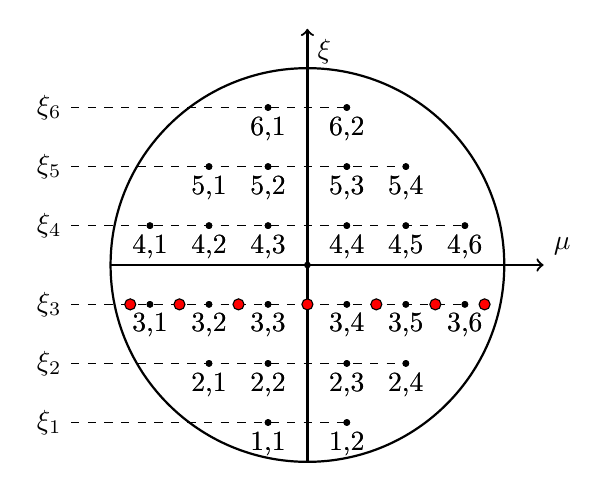
\begin{tikzpicture}[scale=0.5]

\draw[fill=black] (0,0) circle (2pt);
\draw[thick,->] (-5,0) -- (6,0) node[above right]{$\mu$};
\draw[thick,->] (0,-5) -- (0,6) node[below right]{$\xi$};
\draw[thick] (0,0) circle (5cm);

\draw[dashed] (-6,-4) node[left]{$\xi_1$} -- (1,-4);
\draw[dashed] (-6,-2.5) node[left]{$\xi_2$} -- (2.5,-2.5);
\draw[dashed] (-6,-1) node[left]{$\xi_3$} -- (4,-1);
\draw[dashed] (-6,1) node[left]{$\xi_4$} -- (4,1);
\draw[dashed] (-6,2.5) node[left]{$\xi_5$} -- (2.5,2.5);
\draw[dashed] (-6,4) node[left]{$\xi_6$} -- (1,4);

\onslide<1>{
\draw[fill=black] (-4,-1) circle (2pt) node[below]{3,1};
\draw[fill=black] (-2.5,-1) circle (2pt) node[below]{3,2};
\draw[fill=black] (-1,-1) circle (2pt) node[below]{3,3};
\draw[fill=black] (-2.5,-2.5) circle (2pt) node[below]{2,1};
\draw[fill=black] (-1, -2.5) circle (2pt) node[below]{2,2};
\draw[fill=black] (-1,-4) circle (2pt) node[below]{1,1};

\draw[fill=black] (1,-1) circle (2pt) node[below]{3,4};
\draw[fill=black] (2.5,-1) circle (2pt) node[below]{3,5};
\draw[fill=black] (4,-1) circle (2pt) node[below]{3,6};
\draw[fill=black] (1, -2.5) circle (2pt) node[below]{2,3};
\draw[fill=black] (2.5,-2.5) circle (2pt) node[below]{2,4};
\draw[fill=black] (1,-4) circle (2pt) node[below]{1,2};

\draw[fill=black] (-4,1) circle (2pt) node[below]{4,1};
\draw[fill=black] (-2.5,1) circle (2pt) node[below]{4,2};
\draw[fill=black] (-1,1) circle (2pt) node[below]{4,3};
\draw[fill=black] (-2.5,2.5) circle (2pt) node[below]{5,1};
\draw[fill=black] (-1, 2.5) circle (2pt) node[below]{5,2};
\draw[fill=black] (-1,4) circle (2pt) node[below]{6,1};

\draw[fill=black] (1,1) circle (2pt) node[below]{4,4};
\draw[fill=black] (2.5,1) circle (2pt) node[below]{4,5};
\draw[fill=black] (4,1) circle (2pt) node[below]{4,6};
\draw[fill=black] (1, 2.5) circle (2pt) node[below]{5,3};
\draw[fill=black] (2.5,2.5) circle (2pt) node[below]{5,4};
\draw[fill=black] (1,4) circle (2pt) node[below]{6,2};}

\onslide<2->{
\draw[fill=black] (-4,-1) circle (2pt) node[below]{3,1};
\draw[fill=black] (-2.5,-1) circle (2pt) node[below]{3,2};
\draw[fill=black] (-1,-1) circle (2pt) node[below]{3,3};
\draw[fill=black] (-2.5,-2.5) circle (2pt) node[below]{2,1};
\draw[fill=black] (-1, -2.5) circle (2pt) node[below]{2,2};
\draw[fill=black] (-1,-4) circle (2pt) node[below]{1,1};

\draw[fill=black] (1,-1) circle (2pt) node[below]{3,4};
\draw[fill=black] (2.5,-1) circle (2pt) node[below]{3,5};
\draw[fill=black] (4,-1) circle (2pt) node[below]{3,6};
\draw[fill=black] (1, -2.5) circle (2pt) node[below]{2,3};
\draw[fill=black] (2.5,-2.5) circle (2pt) node[below]{2,4};
\draw[fill=black] (1,-4) circle (2pt) node[below]{1,2};

\draw[fill=black] (-4,1) circle (2pt) node[below]{4,1};
\draw[fill=black] (-2.5,1) circle (2pt) node[below]{4,2};
\draw[fill=black] (-1,1) circle (2pt) node[below]{4,3};
\draw[fill=black] (-2.5,2.5) circle (2pt) node[below]{5,1};
\draw[fill=black] (-1, 2.5) circle (2pt) node[below]{5,2};
\draw[fill=black] (-1,4) circle (2pt) node[below]{6,1};

\draw[fill=black] (1,1) circle (2pt) node[below]{4,4};
\draw[fill=black] (2.5,1) circle (2pt) node[below]{4,5};
\draw[fill=black] (4,1) circle (2pt) node[below]{4,6};
\draw[fill=black] (1, 2.5) circle (2pt) node[below]{5,3};
\draw[fill=black] (2.5,2.5) circle (2pt) node[below]{5,4};
\draw[fill=black] (1,4) circle (2pt) node[below]{6,2};

%\draw[fill=red] (-4.5,1) circle (4pt) node[below]{$\left(4,\frac{1}{2} \right)$};
%\draw[fill=red] (-3.25,1) circle (4pt) node[below]{$\left(4,\frac{3}{2} \right)$};
%\draw[fill=red] (-1.75,1) circle (4pt) node[below]{$\left(4,\frac{5}{2} \right)$};
%\draw[fill=red] (0,1) circle (4pt) node[below]{$\left(4,\frac{7}{2} \right)$};
%\draw[fill=red] (1.75,1) circle (4pt) node[below]{$\left(4,\frac{9}{2} \right)$};
%\draw[fill=red] (3.25,1) circle (4pt) node[below]{$\left(4,\frac{11}{2} \right)$};
%\draw[fill=red] (4.5,1) circle (4pt) node[below]{$\left(4,\frac{13}{2} \right)$};}

\draw[fill=red] (-4.5,-1) circle (4pt);
\draw[fill=red] (-3.25,-1) circle (4pt);
\draw[fill=red] (-1.75,-1) circle (4pt);
\draw[fill=red] (0,-1) circle (4pt);
\draw[fill=red] (1.75,-1) circle (4pt);
\draw[fill=red] (3.25,-1) circle (4pt);
\draw[fill=red] (4.5,-1) circle (4pt);}

\end{tikzpicture}
\end{figure}

\end{frame}

%%%%%%%%%%%%%%%%%%%%%%%%%%%%%%%%%%%%%%%
\subsection{}
%%%
\begin{frame}
\frametitle{\RZ\ Geometry}
\framesubtitle{Angular derivative approximation - Morel and Montry}

\begin{flalign*}
{\color{blue}- \frac{1}{r} \frac{\partial}{\partial \omega} \eta_{n,m}\ \psi_{n,m} \left(r,z, \vec{\Omega} \right)} & = \frac{\alpha_{m+1/2}^n\ \psi_{n,m+1/2} - \alpha_{m-1/2}^n\ \psi_{n,m-1/2}}{r\ w_{n,m}}
\end{flalign*}
%
\begin{itemize}
\onslide<2->{
\item{Define angular differencing coefficients to preserve uniform infinite medium solution (i.e., $\vec{\Omega} \vd \grad \psi = 0$)}
%
\begin{flalign*}
\alpha_{m+1/2}^n & = \alpha_{m-1/2}^n - \mu_{n,m} w_{n,m} \\
\alpha_{1/2}^n & = \alpha_{M_n+1/2}^n = 0 
\end{flalign*}}
%\onslide<3->{
%\item{Using level-symmetric angular quadrature to sweep through all $\mu_{n,m}$ directions on level $\xi_n$}}
\end{itemize}

\end{frame}

%%%%%%%%%%%%%%%%%%%%%%%%%%%%%%%%%%%%%%%
% Empty subsection required to get the dots to show up in navigation bar
\subsection{}
%%%
\begin{frame}
\frametitle{\RZ\ Geometry}
\framesubtitle{Angular derivative approximation - Morel and Montry}

\begin{itemize}
\item{Weighted diamond difference approximation for $\psi_{n,m}$ between $\psi_{n,m-1/2}$ and $\psi_{n,m+1/2}$, angular fluxes at the boundary of the discrete ordinate direction}
\end{itemize}
%
\begin{flalign*}
\psi_{n,m} & = \tau_{n,m} \psi_{n,m+1/2} + (1-\tau_{n,m}) \psi_{n,m-1/2} \\
\tau_{n,m} & = \frac{\mu_{n,m} - \mu_{n, m+1/2}}{\mu_{n,m+1/2} - \mu_{n,m-1/2}}
\end{flalign*}
\onslide<2->{
\begin{flalign*}
\mu_{n,m+1/2} & = \sqrt{1-\xi_n^2}\ \cos(\gamma_{n,m+1/2}) \\
\gamma_{n,m+1/2} & = \gamma_{n,m-1/2} + \frac{\pi\ w_{n,m}}{\sum\limits_{m=1}^{M_n}  w_{n,m}} \\
\gamma_{n,1/2} & = - \pi
\end{flalign*}}

\end{frame}

%%%%%%%%%%%%%%%%%%%%%%%%%%%%%%%%%%%%%%%
% Empty subsection required to get the dots to show up in navigation bar
\subsection{}
%%%
\begin{frame}
\frametitle{\RZ\ Geometry}
\framesubtitle{Angular derivative approximation - Morel and Montry}

\begin{itemize}
\item{Solve for starting directions $\psi_{n,1/2}$ using Cartesian geometry transport equation}
\end{itemize}
%
\begin{flalign*}
\vec{\Omega} \vd \grad {\color<2>{blue}\psi_{n,1/2}} + \sigma_t\ {\color<2>{blue}\psi_{n,1/2}} & = \frac{1}{2 \pi} \sigma_s\ \phi + \frac{1}{2 \pi} S_0
\end{flalign*}
\onslide<2->{
\begin{itemize}
\item{Relate the starting direction ($m=1/2$) to the first discrete ordinates direction ($m=1$)}
\end{itemize}}
%
\begin{flalign*}
\onslide<2->{
\psi_{n,1} & = \tau_{n,1} {\color<3->{blue}\psi_{n,1+1/2}} + (1-\tau_{n,1}) {\color<2>{blue}\psi_{n,1/2}}} \\
\onslide<3->{
- \frac{1}{r} \frac{\partial}{\partial \omega} \eta\ \psi & = \frac{\alpha_{1+1/2}^n\ {\color{blue}\psi_{n,1+1/2}} - \alpha_{1/2}^n\ \psi_{n,1/2}}{r\ w_{n,1}}}
\end{flalign*}

\end{frame}

%%%%%%%%%%%%%%%%%%%%%%%%%%%%%%%%%%%%%%%
%%%%%%%%%%%%%%%%%%%%%%%%%%%%%%%%%%%%%%%
%%%%%%%%%%%%%%%%%%%%%%%%%%%%%%%%%%%%%%%
%%%%%%%%%%%%%%%%%%%%%%%%%%%%%%%%%%%%%%%
\section{Axisymmetry}
\subsection{}

\begin{frame}
\frametitle{Axisymmetry Preservation}
\framesubtitle{Preserve 1-D spherical symmetry using \RZ\ geometry}

\begin{columns}[T]

\column{0.5\textwidth}
\begin{itemize}
\item{Preserve 1-D spherical symmetry}
\begin{itemize}
\item{only a function of spherical radius, $\rho$}
\end{itemize}
\begin{flalign*}
\rho \equiv \sqrt{r^2+z^2}
\end{flalign*}
\end{itemize}

\begin{figure}
\centering
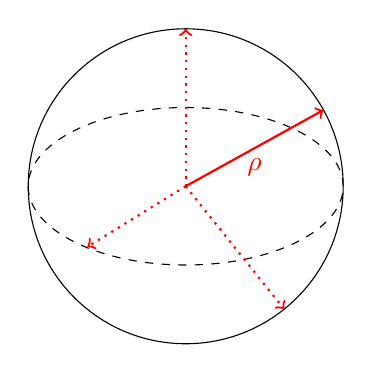
\begin{tikzpicture}
\draw (0,0) circle (2);
\draw[dashed] (0,0) ellipse (2 and 1);
\draw[thick,red,->] (0,0) -- (0.875,0.484) node[anchor=north]{$\rho$} -- (1.75,0.968);

\onslide<2->{\draw[thick,dotted,red,->] (0,0) -- (1.25,-1.56);}
\onslide<3->{\draw[thick,dotted,red,->] (0,0) -- (-1.25,-0.77);}
\onslide<4->{\draw[thick,dotted,red,->] (0,0) -- (0,2);}
\end{tikzpicture}
\end{figure}

\column{0.5\textwidth}
\begin{figure}
\centering
\onslide<5->{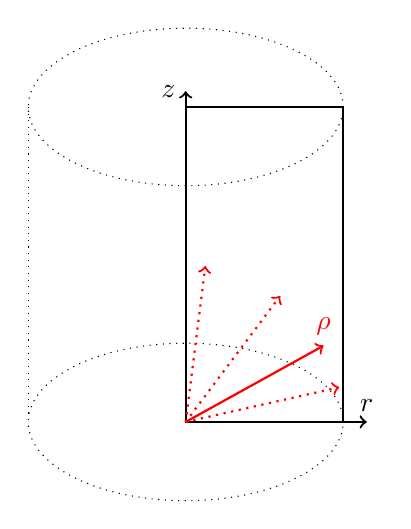
\begin{tikzpicture}
\draw[semithick] (0,0) rectangle (2,4);
\draw[dotted] (0,4) ellipse (2 and 1);
\draw[dotted] (0,0) ellipse (2 and 1);
\draw[dotted] (-2,4) -- (-2,0);

\draw[thick,->] (0,0) -- (2.3,0) node[anchor=south]{$r$};
\draw[thick,->] (0,0) -- (0,4.2) node[anchor=east]{$z$};

\onslide<6->{\draw[thick,red,->] (0,0) -- (0.875,0.484) -- (1.75,0.968) node[anchor=south]{$\rho$};}
\onslide<7->{\draw[thick,dotted,red,->] (0,0) -- (1.95,0.44);}
\onslide<8->{\draw[thick,dotted,red,->] (0,0) -- (1.2,1.6);}
\onslide<9->{\draw[thick,dotted,red,->] (0,0) -- (0.25,1.98);}
\end{tikzpicture}}
\end{figure}


\end{columns}

\end{frame}

%%%%%%%%%%%%%%%%%%%%%%%%%%%%%%%%%%%%%%%
\section{Axisymmetry}
\subsection{}

\begin{frame}
\frametitle{Axisymmetry Preservation}
\framesubtitle{Preserve 1-D spherical symmetry using \RZ\ geometry}

\begin{columns}[T]

\column{0.5\textwidth}
\begin{itemize}
\item{Solve MMS problem with manufactured solution:}
\begin{flalign*}
\psi_\text{MMS} & = \rho \equiv \sqrt{r^2+z^2}
\end{flalign*}
\item{Homogeneous material with $\sigma_t=5.0$, $\sigma_s=2.0$}
\item{Incident angular flux on $\rho=1$ boundary}
\item{Reflecting boundary at $r=0$}
\item{$p=\{1,2,4,8\}$, several $S_N$ orders $(N=\{4,6,8,10,12\})$, $1^\text{st}$- and $2^\text{nd}$-order meshes, several mesh refinements}
\end{itemize}

\column{0.5\textwidth}
\vspace{-10pt}
\begin{figure}
\centering
\only<2>{\includegraphics[scale=0.2,trim={50pt 70pt 320pt 45pt},clip]{../../../Research/graphics/Axisymmetry/RZASMMSLinearRhoBrunner/p1S8g2r5PhiNoContour}}
\only<3>{\includegraphics[scale=0.2,trim={50pt 70pt 320pt 45pt},clip]{../../../Research/graphics/Axisymmetry/RZASMMSLinearRhoBrunner/p1S8g2r5PhiContour}}
\end{figure}

\end{columns}

\end{frame}

%%%%%%%%%%%%%%%%%%%%%%%%%%%%%%%%%%%%%%%
\section{Axisymmetry}
\subsection{}

\begin{frame}
\frametitle{Axisymmetry Preservation}
\framesubtitle{Preserve 1-D spherical symmetry using \RZ\ geometry}

\begin{columns}[T]

\column{0.6\textwidth}
\begin{itemize}
\item{Compare each nodal solution to the average solution at each spherical radius $\rho=\sqrt{r^2+z^2}$}

\begin{flalign*}
\phi_\text{asym}(\rho) & = \left|\frac{\phi_\text{DFEM}(\rho,\theta)- \phi_\text{avg}(\rho)}{\phi_\text{avg}(\rho)} \right| \\
\phi_\text{avg}(\rho) & = \frac{1}{N_\text{nodes}(\rho)} \sum_{i=1}^{N_\text{nodes}(\rho)} \phi_\text{DFEM}(\rho, \theta_i)
\end{flalign*}

\vspace{10pt}

\item{Plot the FEM ``shape'' of $\phi_\text{asym}$}
\end{itemize}

\column{0.4\textwidth}
\vspace{-15pt}
\begin{figure}
\flushright
\begin{tikzpicture}
\node at (0,0){\includegraphics[scale=0.3]{./graphics/RZASNodesRadius.pdf}};
\draw[thick,red,->] (-1.38,0.7) arc (90:30:0.9) node[anchor=south west]{$\theta$};
\end{tikzpicture}
\end{figure}

\end{columns}

\end{frame}

%%%%%%%%%%%%%%%%%%%%%%%%%%%%%%%%%%%%%%%
\section{Axisymmetry}
\subsection{}

\begin{frame}
\frametitle{Axisymmetry Preservation}
\framesubtitle{Relative asymmetry for \underline{$1^\text{st}$-order finite elements} on a \underline{$1^\text{st}$-order mesh} for given order of level-symmetric angular quadrature}

\begin{figure}
\centering
\begin{subfigure}{0.33\textwidth}
\centering
\includegraphics[scale=0.15,trim={50pt 70pt 320pt 45pt},clip]{../../../Research/graphics/Axisymmetry/RZASMMSLinearRhoBrunner/p1S4g1r2}
\caption{$S_4$}
\end{subfigure}%
\begin{subfigure}{0.33\textwidth}
\centering
\includegraphics[scale=0.15,trim={50pt 70pt 320pt 45pt},clip]{../../../Research/graphics/Axisymmetry/RZASMMSLinearRhoBrunner/p1S8g1r2}
\caption{$S_8$}
\end{subfigure}%
\begin{subfigure}{0.33\textwidth}
\centering
\includegraphics[scale=0.15,trim={50pt 70pt 320pt 45pt},clip]{../../../Research/graphics/Axisymmetry/RZASMMSLinearRhoBrunner/p1S12g1r2}
\caption{$S_{12}$}
\end{subfigure}
\end{figure}

\end{frame}

%%%%%%%%%%%%%%%%%%%%%%%%%%%%%%%%%%%%%%%
\section{Axisymmetry}
\subsection{}

\begin{frame}[t]
\frametitle{Axisymmetry Preservation}
\framesubtitle{Relative asymmetry for \underline{$1^\text{st}$-order finite elements} on a \underline{$1^\text{st}$-order mesh} for given order of level-symmetric angular quadrature}

\begin{columns}[T]

\begin{column}{0.4\textwidth}
\begin{itemize}
\item{Difficult to distinguish between $S_N$ solutions}
\item{Greatest asymmetry near origin}
\item{Asymmetry reaches an asymptotic value \textasciitilde$10^{-3}$}
\item{Accuracy of solution is nearly constant}
\end{itemize}

\end{column}

\begin{column}{0.6\textwidth}
\begin{figure}
\flushright
\includegraphics[scale=0.6]{./graphics/RZASMMSLinearRhoBrunnerp1g1r2.pdf}
\end{figure}

\end{column}

\end{columns}

\end{frame}

%%%%%%%%%%%%%%%%%%%%%%%%%%%%%%%%%%%%%%%
\section{Axisymmetry}
\subsection{}

\begin{frame}
\frametitle{Axisymmetry Preservation}
\framesubtitle{Relative asymmetry for \underline{$4^\text{th}$-order finite elements} on a \underline{$1^\text{st}$-order mesh} for given order of level-symmetric angular quadrature}

\begin{figure}
\centering
\begin{subfigure}{0.33\textwidth}
\centering
\includegraphics[scale=0.15,trim={50pt 70pt 320pt 45pt},clip]{../../../Research/graphics/Axisymmetry/RZASMMSLinearRhoBrunner/p4S4g1r2}
\caption{$S_4$}
\end{subfigure}%
\begin{subfigure}{0.33\textwidth}
\centering
\includegraphics[scale=0.15,trim={50pt 70pt 320pt 45pt},clip]{../../../Research/graphics/Axisymmetry/RZASMMSLinearRhoBrunner/p4S8g1r2}
\caption{$S_8$}
\end{subfigure}%
\begin{subfigure}{0.33\textwidth}
\centering
\includegraphics[scale=0.15,trim={50pt 70pt 320pt 45pt},clip]{../../../Research/graphics/Axisymmetry/RZASMMSLinearRhoBrunner/p4S12g1r2}
\caption{$S_{12}$}
\end{subfigure}
\end{figure}

\end{frame}

%%%%%%%%%%%%%%%%%%%%%%%%%%%%%%%%%%%%%%%
\section{Axisymmetry}
\subsection{}

\begin{frame}[t]
\frametitle{Axisymmetry Preservation}
\framesubtitle{Relative asymmetry for \underline{$4^\text{th}$-order finite elements} on a \underline{$1^\text{st}$-order mesh} for given order of level-symmetric angular quadrature}

\begin{columns}[T]

\begin{column}{0.4\textwidth}
\begin{itemize}
\item{Difficult to distinguish between $S_N$ solutions}
\item{Greatest asymmetry near origin}
\item{Asymmetry does not reach an asymptotic value $(<10^{-9})$}
\item{Accuracy of solution is nearly constant}
\end{itemize}

\end{column}

\begin{column}{0.6\textwidth}
\begin{figure}
\flushright
\includegraphics[scale=0.6]{./graphics/RZASMMSLinearRhoBrunnerp4g1r2.pdf}
\end{figure}

\end{column}

\end{columns}

\end{frame}

%%%%%%%%%%%%%%%%%%%%%%%%%%%%%%%%%%%%%%%
\section{Axisymmetry}
\subsection{}

\begin{frame}[t]
\frametitle{Axisymmetry Preservation}
\framesubtitle{Relative asymmetries for each finite element order on a \underline{$1^\text{st}$-order mesh} for $S_8$ level-symmetric angular quadrature}

\begin{columns}[T]

\begin{column}{0.4\textwidth}
\begin{itemize}
\item{$1^\text{st}$- and $2^\text{nd}$-order finite elements reach asymptotic asymmetry}
\item{Increasing finite element order increases relative symmetry}
\item{Asymmetry does not reach an asymptotic value $(<10^{-9})$ for higher-order finite elements}
\item{Relative symmetry is nearly identical at the origin}
\end{itemize}

\end{column}

\begin{column}{0.6\textwidth}
\begin{figure}
\flushright
\includegraphics[scale=0.6]{./graphics/RZASMMSLinearRhoBrunnerS8g1r2.pdf}
\end{figure}

\end{column}

\end{columns}

\end{frame}

%%%%%%%%%%%%%%%%%%%%%%%%%%%%%%%%%%%%%%%
\section{Axisymmetry}
\subsection{}

\begin{frame}
\frametitle{Axisymmetry Preservation}
\framesubtitle{Relative asymmetry under spatial refinement for \underline{$4^\text{th}$-order finite elements} on a \underline{$1^\text{st}$-order mesh} for given order of level-symmetric angular quadrature}

\begin{figure}
\centering
\begin{subfigure}{0.33\textwidth}
\centering
\includegraphics[scale=0.15,trim={50pt 70pt 320pt 45pt},clip]{../../../Research/graphics/Axisymmetry/RZASMMSLinearRhoBrunner/p4S8g1r1CompR}
\caption{28 zones}
\end{subfigure}%
\begin{subfigure}{0.33\textwidth}
\centering
\includegraphics[scale=0.15,trim={50pt 70pt 320pt 45pt},clip]{../../../Research/graphics/Axisymmetry/RZASMMSLinearRhoBrunner/p4S8g1r3CompR}
\caption{496 zones}
\end{subfigure}%
\begin{subfigure}{0.33\textwidth}
\centering
\includegraphics[scale=0.15,trim={50pt 70pt 320pt 45pt},clip]{../../../Research/graphics/Axisymmetry/RZASMMSLinearRhoBrunner/p4S8g1r5CompR}
\caption{8128 zones}
\end{subfigure}
\end{figure}

\end{frame}

%%%%%%%%%%%%%%%%%%%%%%%%%%%%%%%%%%%%%%%
\section{Axisymmetry}
\subsection{}

\begin{frame}[t]
\frametitle{Axisymmetry Preservation}
\framesubtitle{Relative asymmetries under spatial refinement for \underline{$4^\text{st}$-order finite elements} on a \underline{$1^\text{st}$-order mesh} for $S_8$ level-symmetric angular quadrature}

\begin{columns}[T]

\begin{column}{0.4\textwidth}
\begin{itemize}
\item{Mesh refinement increases symmetry preservation}
\item{Largest magnitude asymmetries are located near the origin}
\item{Mesh refinement increases accuracy of scalar flux}
\end{itemize}

\end{column}

\begin{column}{0.6\textwidth}
\begin{figure}
\flushright
\includegraphics[scale=0.6]{./graphics/RZASMMSLinearRhoBrunnerp4S8g1.pdf}
\end{figure}

\end{column}

\end{columns}

\end{frame}

%%%%%%%%%%%%%%%%%%%%%%%%%%%%%%%%%%%%%%%
%%%%%%%%%%%%%%%%%%%%%%%%%%%%%%%%%%%%%%%
%%%%%%%%%%%%%%%%%%%%%%%%%%%%%%%%%%%%%%%
%%%%%%%%%%%%%%%%%%%%%%%%%%%%%%%%%%%%%%%
\section{Axisymmetry}
\subsection{}

\begin{frame}
\frametitle{Axisymmetry Preservation}
\framesubtitle{Relative asymmetry for \underline{$1^\text{st}$-order finite elements} on a \underline{$2^\text{nd}$-order mesh} for given order of level-symmetric angular quadrature}

\begin{figure}
\centering
\begin{subfigure}{0.33\textwidth}
\centering
\includegraphics[scale=0.15,trim={50pt 70pt 320pt 45pt},clip]{../../../Research/graphics/Axisymmetry/RZASMMSLinearRhoBrunner/p1S4g2r2}
\caption{$S_4$}
\end{subfigure}%
\begin{subfigure}{0.33\textwidth}
\centering
\includegraphics[scale=0.15,trim={50pt 70pt 320pt 45pt},clip]{../../../Research/graphics/Axisymmetry/RZASMMSLinearRhoBrunner/p1S8g2r2}
\caption{$S_8$}
\end{subfigure}%
\begin{subfigure}{0.33\textwidth}
\centering
\includegraphics[scale=0.15,trim={50pt 70pt 320pt 45pt},clip]{../../../Research/graphics/Axisymmetry/RZASMMSLinearRhoBrunner/p1S12g2r2}
\caption{$S_{12}$}
\end{subfigure}
\end{figure}

\end{frame}

%%%%%%%%%%%%%%%%%%%%%%%%%%%%%%%%%%%%%%%
\section{Axisymmetry}
\subsection{}

\begin{frame}[t]
\frametitle{Axisymmetry Preservation}
\framesubtitle{Relative asymmetry for \underline{$1^\text{st}$-order finite elements} on a \underline{$2^\text{nd}$-order mesh} for given order of level-symmetric angular quadrature}

\begin{columns}[T]

\begin{column}{0.4\textwidth}
\begin{itemize}
\item{Difficult to distinguish between $S_N$ solutions}
\item{Greatest asymmetry near origin}
\item{Asymmetry does not reach an asymptotic value $(<10^{-6})$}
\item{Accuracy is nearly constant}
\end{itemize}

\end{column}

\begin{column}{0.6\textwidth}
\begin{figure}
\flushright
\includegraphics[scale=0.6]{./graphics/RZASMMSLinearRhoBrunnerp1g2r2.pdf}
\end{figure}

\end{column}

\end{columns}

\end{frame}

%%%%%%%%%%%%%%%%%%%%%%%%%%%%%%%%%%%%%%%
%%%%%%%%%%%%%%%%%%%%%%%%%%%%%%%%%%%%%%%
%%%%%%%%%%%%%%%%%%%%%%%%%%%%%%%%%%%%%%%
%%%%%%%%%%%%%%%%%%%%%%%%%%%%%%%%%%%%%%%
\section{Conclusions}
\subsection{}

\begin{frame}
\frametitle{MIP DSA Conclusions}

\begin{itemize}
\item{Implemented MIP DSA equations with \ul{Robin} boundary conditions}
\begin{itemize}
\item{Unconditionally converging}
\item{Greatly accelerates source iteration}
\end{itemize}
\item{Compared spectral radii to the MIP DSA equations with \ul{Dirichlet} boundary conditions}
\begin{itemize}
\item{Robin BCs do not generate the peaks}
\item{Robin BCs are not as dependent on the constant $C$ or $p$}
\item{Robin BCs have significantly higher spectral radii in optically thick region}
\end{itemize}
\item{Future work}
\begin{itemize}
\item{Investigate the optically thick region}
\item{Fourier analysis}
\item{Implement MIP DSA in a preconditioned Krylov method}
\end{itemize}
\end{itemize}

\end{frame}

%%%%%%%%%%%%%%%%%%%%%%%%%%%%%%%%%%%%%%%
\section{Conclusions}
\subsection{}
\begin{frame}
\frametitle{\RZ\ Geometry Conclusions}

\begin{itemize}
\item{Implemented and characterized the \RZ\ spatial discretization using HO finite elements on meshes with curved surfaces}
\item{Observed expected $O(p+1)$ spatial convergence rates on smooth solutions}
\item{Curvature of the mesh does not degrade spatial convergence}
%\item{Strong heterogeneities introduce oscillations}
%\item{Unresolved boundary layers introduce oscillations}
\item{Axisymmtery preservation is conditional with two dominant factors:}
\begin{itemize}
\item{spatial mesh refinement}
\item{finite element order}
\end{itemize}
\item{Future work}
\begin{itemize}
\item{Numerically demonstrate diffusion limit}
\item{Consider alternate derivations of \RZ\ equations}
\item{Consider other manufactured solutions and materials for symmetry preservation}
\end{itemize}
%\item{Weighted diamond differencing the angular derivative cannot resolve $\mu^2$ dependency}
%\begin{itemize}
%\item{Increasing angular quadrature order may better resolve linear dependency}
%\end{itemize}
\end{itemize}

\end{frame}

%%%%%%%%%%%%%%%%%%%%%%%%%%%%%%%%%%%%%%%
\section{Thank You}
\subsection{}

\begin{frame}
\frametitle{}

\vspace{50pt}
\begin{center}
\huge{Thank you!}
\end{center}

\centering
\includegraphics[width=0.4\textwidth]{./osu_img/beaverlogo}

\end{frame}




%%%%%%%%%%%%%%%%%%%%%%%%%%%%%%%%%%%%%%%
%%%%%%%%%%%%%%%%%%%%%%%%%%%%%%%%%%%%%%%
%%%%%%%%%%%%%%%%%%%%%%%%%%%%%%%%%%%%%%%
\appendix	
\subsection{}

\begin{frame}
\frametitle{\XY\ Geometry}
\framesubtitle{Spatial convergence study}

\begin{itemize}
\item{Method of manufactured solutions (MMS) to determine convergence rates}
{\small
\begin{flalign*}
\psi_\text{MMS} & = \left(1-\mu^2 \right) \left(1-\eta^2 \right) \sin(4 \pi x) \cos \left(\frac{7}{2} \pi y \right)
\end{flalign*}}
\end{itemize}

\begin{columns}[T]

\column{0.6\textwidth}
\begin{itemize}
\item{Calculate $\norm{\phi_\text{code} - \phi_\text{MMS}}_{L^2}$ for sequential mesh refinements}
\item{Use $p=\{1,2,4,6,8\}$}
\item{Orthogonal and $3^\text{rd}$-order meshes}
\end{itemize}

\column{0.4\textwidth}
\vspace{0pt}
\begin{figure}
\includegraphics[width=\textwidth,trim={50pt 10pt 50pt 60pt},clip]{../../../Research/graphics/GleicherMMS_a4_b72}
\end{figure}

\end{columns}

\end{frame}

%%%%%%%%%%%%%%%%%%%%%%%%%%%%%%%%%%%%%%%
\subsection{}

\begin{frame}
\frametitle{\XY\ Geometry}
\framesubtitle{Spatial convergence study shows $p+1$ convergence}

\begin{itemize}
\item{$N_\text{unknowns} = N_\text{cells} (p+1)^2$}
\item{Reference lines show $p+1$ spatial convergences}
\end{itemize}

\vspace{-15pt}

\begin{figure}
\centering
\small
\begin{subfigure}{0.5\textwidth}
\begin{tikzpicture}
  \begin{axis}[
    width=0.95\textwidth,
    height=0.55\textheight,
    grid=major,
    xlabel={$\sqrt{\text{N}_\text{unknowns}}$},
    ylabel={L$^2$-error},
  	xmode=log,
  	ymode=log,
  	xmin=8,xmax=1e3,
  	ymin=1e-15,ymax=1e1,
  	]
\addplot[mark=*, mark size=2, only marks, draw=black, mark options={solid, fill=black}] table [x=ne1, y=fe1]{./graphics/GleicherMMSOrthoa4b72.dat};
\addplot[mark=triangle*, only marks, mark size=3, draw=red, mark options={solid, fill=red}] table [x=ne2, y=fe2]{./graphics/GleicherMMSOrthoa4b72.dat};
\addplot[mark=square*, only marks, mark size=2, draw=blue, mark options={solid, fill=blue}] table [x=ne4, y=fe4]{./graphics/GleicherMMSOrthoa4b72.dat};
\addplot[mark=diamond*, only marks, mark size=3, draw=magenta, mark options={solid, fill=magenta}] table [x=ne6, y=fe6]{./graphics/GleicherMMSOrthoa4b72.dat};
\addplot[mark=star, only marks, mark size=3, draw=orange, mark options={solid, fill=orange}] table [x=ne8, y=fe8]{./graphics/GleicherMMSOrthoa4b72.dat};

\addplot[black] table[row sep=crcr] {
8 2 \\
256 0.002 \\};
\addplot[red] table[row sep=crcr] {
12 0.2 \\
384 6.1035e-06 \\};
\addplot[blue] table[row sep=crcr] {
20	1e-2 \\
320	9.5367e-09 \\};
\addplot[magenta] table[row sep=crcr] {
28	1e-4 \\
224	4.7684e-11 \\};
\addplot[orange] table[row sep=crcr] {
36	1e-6 \\
288	7.4506e-15 \\};

  \end{axis}
\end{tikzpicture}
\centering
{\footnotesize Orthogonal mesh}
\end{subfigure}%
\begin{subfigure}{0.5\textwidth}
\begin{tikzpicture}
  \begin{axis}[
    width=0.95\textwidth,
    height=0.55\textheight,
    grid=major,
    xlabel={$\sqrt{\text{N}_\text{unknowns}}$},
    ylabel={L$^2$-error},
  	xmode=log,
  	ymode=log,
  	xmin=8,xmax=1e3,
  	ymin=1e-15,ymax=1e1,
  	legend style={at={(1.3,1.0)},anchor=north east},
  	]
\addplot[mark=*, only marks, mark size=2, draw=black, mark options={solid, fill=black}] table [x=ne1, y=fe1]{./graphics/GleicherMMS3Mesha4b72.dat};
\addlegendentry{$p=1$}
\addplot[mark=triangle*, only marks, mark size=3, draw=red, mark options={solid, fill=red}] table [x=ne2, y=fe2]{./graphics/GleicherMMS3Mesha4b72.dat};
\addlegendentry{$p=2$}
\addplot[mark=square*, only marks, mark size=2, draw=blue, mark options={solid, fill=blue}] table [x=ne4, y=fe4]{./graphics/GleicherMMS3Mesha4b72.dat};
\addlegendentry{$p=4$}
\addplot[mark=diamond*, only marks, mark size=3, draw=magenta, mark options={solid, fill=magenta}] table [x=ne6, y=fe6]{./graphics/GleicherMMS3Mesha4b72.dat};
\addlegendentry{$p=6$}
\addplot[mark=star, only marks, mark size=3, draw=orange, mark options={solid, fill=orange}] table [x=ne8, y=fe8]{./graphics/GleicherMMS3Mesha4b72.dat};
\addlegendentry{$p=8$}

\addplot[black] table[row sep=crcr] {
8 2 \\
256 0.002 \\};
\addplot[red] table[row sep=crcr] {
12 0.2 \\
384 6.1035e-06 \\};
\addplot[blue] table[row sep=crcr] {
20	3e-2 \\
320	2.8610e-08 \\};
\addplot[magenta] table[row sep=crcr] {
28	2e-3 \\
224	9.5367e-10 \\};
\addplot[orange] table[row sep=crcr] {
36	1e-4 \\
144	3.8147e-10 \\};

  \end{axis}
\end{tikzpicture}
\centering
{\footnotesize $3^\text{rd}$-order mesh}
\end{subfigure}
\end{figure}

\end{frame}

%%%%%%%%%%%%%%%%%%%%%%%%%%%%%%%%%%%%%%%%%%%
\subsection{}

\begin{frame}
\frametitle{\XY\ Geometry}
\framesubtitle{Strong material heterogeneity problem definition}

\vspace{-10pt}

\begin{columns}[T]

\column{0.35\textwidth}
\begin{table}[!h]
\tiny
\centering
{\renewcommand{\arraystretch}{1.5}
\begin{tabular}{|c|c|c|}
\hline
Material Region & $\sigma_t$ cm$^{-1}$ & $\sigma_s$ cm$^{-1}$ \\
\hline
Source & 1.0 & 1.0 \\
Very thin absorber & 0.0001 & 0.0 \\
Thick absorber & 10.0 & 0.0 \\
Very thick absorber & 100.0 & 0.0 \\
Very thick scatterer & 1000.0 & 1000.0 \\
\hline
\end{tabular}}
\end{table}

\begin{itemize}
\item{Designed to test optical thicknesses ranging several orders of magnitude}
\item{Create anisotropic fluxes into scattering region}
\end{itemize}

\column{0.65\textwidth}
\begin{figure}[!h]
\tiny
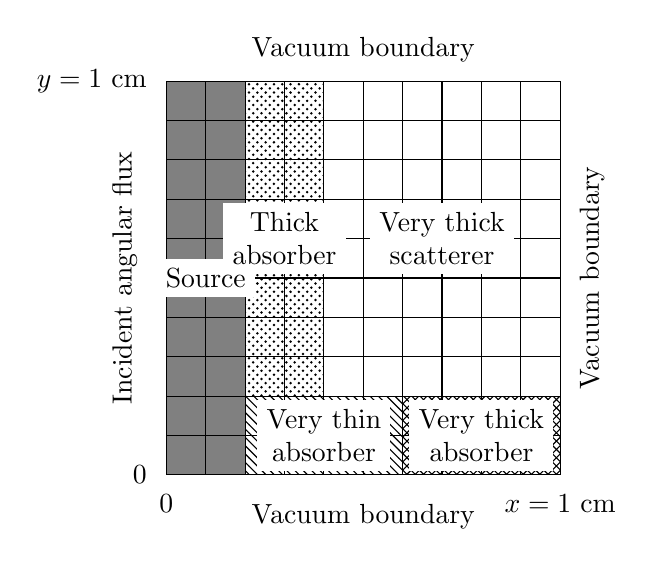
\begin{tikzpicture}[scale=0.5]
\node [below] at (0,-0.25) {0};
\node [left] at (-0.25,0) {0};
\node [left] at (-0.25,10) {$y = 1$ cm};
\node [below] at (10,-0.25) {$x = 1$ cm};
\node [below] at (5,-0.5) {Vacuum boundary};
\node [above] at (5,10.25) {Vacuum boundary};
\node [right] at (10.25,5) {\rotatebox{90}{Vacuum boundary}};
\node [left] at (-0.5,5) {\rotatebox{90}{Incident angular flux}};
\draw [fill=gray] (0,0) rectangle (2,10);
\draw [pattern= north west lines] (2,0) rectangle (6,2);
\draw [pattern=crosshatch dots] (2,2) rectangle (4,10);
\draw [pattern=crosshatch] (6,0) rectangle (10,2);
\draw (0,0) grid (10,10);
\node [fill=white] at (1,5) {Source};
\node [align=center,fill=white] at (4,1) {Very thin\\absorber};
\node [align=center,fill=white] at (3,6) {Thick\\absorber};
\node [align=center,fill=white] at (8,1) {Very thick\\absorber};
\node [align=center,fill=white] at (7,6) {Very thick\\scatterer};
\end{tikzpicture}
\end{figure}

\end{columns}

\end{frame}

%%%%%%%%%%%%%%%%%%%%%%%%%%%%%%%%%%%%%%%%%%%
\section{XY Geometry}
\subsection{}

\begin{frame}
\frametitle{\XY\ Geometry}
\framesubtitle{Strong material heterogeneity problem results}

\begin{columns}[T]
\column{0.5\textwidth}
\begin{figure}[!h]
\centering
\includegraphics[width=\textwidth,trim={50pt 70pt 45pt 45pt},clip]{../../../Research/graphics/TP3S8e8MIPDSAC2Current}
\flushleft\tiny{Multi-material stress test solved with Robin BC MIP DSA. White regions indicate negative energy density.}
\label{fig:TP3DSA}
\end{figure}

\column{0.5\textwidth}
\begin{figure}[!h]
\centering
\includegraphics[width=\textwidth,trim={50pt 70pt 45pt 45pt},clip]{../../../Research/graphics/TP3S8e8MIPDSAC2CurrentLog}
\flushleft\tiny{Log of multi-material stress test solved with Robin BC MIP DSA. White regions indicate negative energy density.}
\label{fig:TP3DSAlog}
\end{figure}
\end{columns}

\end{frame}

%%%%%%%%%%%%%%%%%%%%%%%%%%%%%%%%%%%%%%%
%%%%%%%%%%%%%%%%%%%%%%%%%%%%%%%%%%%%%%%
%%%%%%%%%%%%%%%%%%%%%%%%%%%%%%%%%%%%%%%
%%%%%%%%%%%%%%%%%%%%%%%%%%%%%%%%%%%%%%%
% Empty subsection required to get the dots to show up in navigation bar
\subsection{}
\begin{frame}
\frametitle{\RZ\ Geometry}
\framesubtitle{MMS spatial convergence study}

{\small
$\psi_\text{MMS} = (\sin(\pi r)+1-r) \sin(\pi z)$}

\begin{columns}[T]

\column{0.35\textwidth}
\begin{itemize}
\item{Bailey et al. demonstrated $2^\text{nd}$-order convergence for PWL and BLD}
\item{We solve using $p=\{1,2,4,6,8\}$ on an orthogonal and $2^\text{nd}$-order curved mesh}
\item{$S_8$ level-symmetric angular quadrature}
\end{itemize}

\column{0.6\textwidth}
\includegraphics[scale=0.2,trim={50pt 70pt 50pt 40pt},clip]{../../../Research/graphics/RZBaileyS4O2R2D2}

\end{columns}

\end{frame}

%%%%%%%%%%%%%%%%%%%%%%%%%%%%%%%%%%%%%%%
% Empty subsection required to get the dots to show up in navigation bar
\subsection{}
\begin{frame}
\frametitle{\RZ\ Geometry}
\framesubtitle{MMS spatial convergence study shows $p+1$ convergence}

\begin{itemize}
\item{$N_\text{unknowns} = N_\text{cells} (p+1)^2$}
\item{Reference lines show $p+1$ spatial convergences}
\end{itemize}

\vspace{-10pt}

\begin{figure}[!htb]
\centering
\hspace{-30pt}
\begin{subfigure}{0.5\textwidth}
\footnotesize
\flushleft
\begin{tikzpicture}
  \begin{axis}[
    width=0.95\textwidth,
    height=0.55\textheight,
    grid=major,
    xlabel={$\sqrt{\text{N}_\text{unknowns}}$},
    ylabel={L$^2$ error},
  	xmode=log,
  	ymode=log,
  	xmin=8,xmax=1e3,
  	ymin=1e-16,ymax=1e1,
  	]

\addplot[mark=*, mark size=2, only marks, draw=black, mark options={solid, fill=black}] table [x=un1, y=fe1]{../../../Research/graphics/RZBaileyMMSS4D0.dat};
\addplot[mark=triangle*, only marks, mark size=3, draw=red, mark options={solid, fill=red}] table [x=un2, y=fe2]{../../../Research/graphics/RZBaileyMMSS4D0.dat};
\addplot[mark=square*, only marks, mark size=2, draw=blue, mark options={solid, fill=blue}] table [x=un4, y=fe4]{../../../Research/graphics/RZBaileyMMSS4D0.dat};
\addplot[mark=diamond*, only marks, mark size=2, draw=magenta, mark options={solid, fill=magenta}] table [x=un6, y=fe6]{../../../Research/graphics/RZBaileyMMSS4D0.dat};
\addplot[mark=star, only marks, mark size=2, draw=orange, mark options={solid, fill=orange}] table [x=un8, y=fe8]{../../../Research/graphics/RZBaileyMMSS4D0.dat};

\addplot[black] table[row sep=crcr] {
8 0.1 \\
256 9.7656e-05 \\};
\addplot[red] table[row sep=crcr] {
12 0.005 \\
384 1.5259e-07 \\};
\addplot[blue] table[row sep=crcr] {
20	3e-5 \\
320	2.8610e-11 \\};
\addplot[magenta] table[row sep=crcr] {
28	4e-8 \\
224	1.9073e-14 \\};
\addplot[orange] table[row sep=crcr] {
36	5e-11 \\
144	1.9073e-16 \\};

  \end{axis}
\end{tikzpicture}
\centering
{\footnotesize Orthogonal mesh}
\end{subfigure}%
\begin{subfigure}{0.5\textwidth}
\flushleft
\footnotesize
\begin{tikzpicture}
  \begin{axis}[
    width=0.95\textwidth,
    height=0.55\textheight,
    grid=major,
    xlabel={$\sqrt{\text{N}_\text{unknowns}}$},
    ylabel={L$^2$ error},
  	xmode=log,
  	ymode=log,
  	xmin=8,xmax=1e3,
  	ymin=1e-16,ymax=1e1,
  	legend style={at={(1.2,1.0)},anchor=north east},
  	]
\addplot[mark=*, mark size=2, only marks, draw=black, mark options={solid, fill=black}] table [x=un1, y=fe1]{../../../Research/graphics/RZBaileyMMSS4D2.dat};
\addlegendentry{$p=1$}
\addplot[mark=triangle*, only marks, mark size=3, draw=red, mark options={solid, fill=red}] table [x=un2, y=fe2]{../../../Research/graphics/RZBaileyMMSS4D2.dat};
\addlegendentry{$p=2$}
\addplot[mark=square*, only marks, mark size=2, draw=blue, mark options={solid, fill=blue}] table [x=un4, y=fe4]{../../../Research/graphics/RZBaileyMMSS4D2.dat};
\addlegendentry{$p=4$}
\addplot[mark=diamond*, only marks, mark size=2, draw=magenta, mark options={solid, fill=magenta}] table [x=un6, y=fe6]{../../../Research/graphics/RZBaileyMMSS4D2.dat};
\addlegendentry{$p=6$}
\addplot[mark=star, only marks, mark size=2, draw=orange, mark options={solid, fill=orange}] table [x=un8, y=fe8]{../../../Research/graphics/RZBaileyMMSS4D2.dat};
\addlegendentry{$p=8$}

\addplot[black] table[row sep=crcr] {
8 0.3 \\
256 2.9297e-04 \\};
\addplot[red] table[row sep=crcr] {
12 0.01 \\
384 3.0518e-07 \\};
\addplot[blue] table[row sep=crcr] {
20	3e-4 \\
320	2.8610e-10 \\};
\addplot[magenta] table[row sep=crcr] {
28	4e-6 \\
224	1.9073e-12 \\};
\addplot[orange] table[row sep=crcr] {
36	1e-8 \\
144	3.8147e-14 \\};

  \end{axis}
\end{tikzpicture}
\centering
{\footnotesize $2^\text{nd}$-order curved mesh}
\end{subfigure}
\end{figure}

\end{frame}

%%%%%%%%%%%%%%%%%%%%%%%%%%%%%%%%%%%%%%%
\subsection{}

\begin{frame}
\frametitle{\RZ\ Geometry}
\framesubtitle{Regularity constrained spatial convergence study shows $O(3/2)$ convergence rates}

\begin{columns}[T]

\column{0.6\textwidth}
\begin{itemize}
\item{Method of manufactured solutions (MMS) to determine convergence rates}
\begin{flalign*}
\psi_\text{MMS} & =
\begin{cases}
1.0 + 4.0 r, & 0 \leq r < 0.33 \\
3.31 - 3.0 r, & 0.33 \leq r < 0.66 \\
2.32 - 1.5 r, & r \leq 1.0
\end{cases}
\end{flalign*}
\item{Calculate $\norm{\phi_\text{code} - \phi_\text{MMS}}_{L^2}$ for sequential mesh refinements}
\item{Use $p=\{1,2,4\}$, $S_{12}$ level-symmetric angular quadrature, $2^\text{nd}$-order mesh}
\end{itemize}

\column{0.4\textwidth}
\only<1>{
\begin{figure}
\centering
\includegraphics[scale=0.15,trim={50pt 160pt 60pt 50pt},clip]{../../../Research/graphics/RZDiscontRp2S12g2r3}
\end{figure}}

\only<2>{
\begin{figure}[!htb]
\centering
\footnotesize
\begin{tikzpicture}
  \begin{axis}[
    width=\textwidth,
    %height=0.9\textwidth,
    grid=major,
    xlabel={$\sqrt{\text{N}_\text{unknowns}}$},
    ylabel={L$^2$ error},
  	xmode=log,
  	ymode=log,
  	xmin=10,xmax=7e2,
  	ymin=1e-3,ymax=1e1,
  	legend style={at={(1,2)},anchor=north east},
  	]

\addplot[mark=triangle*, only marks, mark size=3, draw=red, mark options={solid, fill=red}] table[row sep=crcr] {
12 0.822493 \\
24 0.43734036 \\
48 0.076831588 \\
96 0.037120875 \\
192 0.014887499 \\
384 0.0050662591 \\};
\addlegendentry{$p=1$}
\addplot[mark=*, mark size=2, only marks, draw=black, mark options={solid, fill=black}] table[row sep=crcr] {
12 0.60652325 \\
24 0.21194424 \\
48 0.047687556 \\
96 0.018428546 \\
192 0.009601399 \\
384 0.0029490701 \\};
\addlegendentry{$p=2$}
\addplot[mark=square*, only marks, mark size=2, draw=blue, mark options={solid, fill=blue}] table[row sep=crcr] {
12 0.36159159 \\
24 0.090767945 \\
48 0.02399935 \\
96 0.011502376 \\
192 0.0045548581 \\
384 0.0029490701 \\};
\addlegendentry{$p=4$}

\addplot[dashed,black] table[row sep=crcr] {
12 1.2 \\
384 0.0066 \\};
\addlegendentry{$O \left(\left(\sqrt{N_\text{un}} \right)^{3/2} \right)$}

  \end{axis}
\end{tikzpicture}
\end{figure}}

\end{columns}

\end{frame}

%%%%%%%%%%%%%%%%%%%%%%%%%%%%%%%%%%%%%%%%%%%
\subsection{}

\begin{frame}
\frametitle{\RZ\ Geometry}
\framesubtitle{Strong scatter with alternating boundary conditions}

\begin{columns}[T]

\column{0.5\textwidth}
\begin{itemize}
\item{Incident flux boundary at gray cells $\psi_\text{inc}=2/\pi$}
\item{$\sigma_t = 1000$, $\sigma_s = 999$, $S_0 = 0$}
\item{$4^\text{th}$-order finite elements}
\item{Designed to reveal boundary layer}
\end{itemize}

\column{0.5\textwidth}
\vspace{-10pt}
\begin{figure}[!h]
\tiny
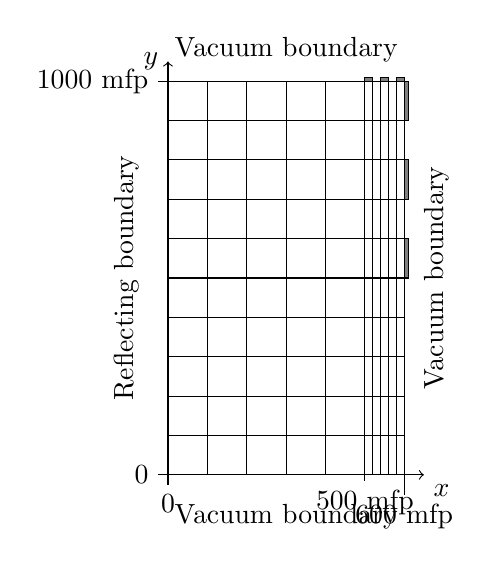
\begin{tikzpicture}[scale=0.5]
\draw [->] (0,0) -- (6.5,0);
\draw [->] (0,0) -- (0,10.5);
\node [left] at (0,10.5) {$y$};
\node [below right] at (6.5,0) {$x$};
\draw (0,-0.25) -- (0,0) -- (-0.25,0);
\draw (5,0) -- (5,-0.15);
\draw (6,0) -- (6,-0.5);
\draw (0,10) -- (-0.25,10);
\node [below] at (0,-0.25) {0};
\node [left] at (-0.25,0) {0};
\node [below] at (5,-0.15) {500 mfp};
\node [below] at (6,-0.5) {600 mfp};
\node [left] at (-0.25,10) {1000 mfp};
\node [below] at (3,-0.5) {Vacuum boundary};
\node [above] at (3,10.25) {Vacuum boundary};
\node [right] at (6.25,5) {\rotatebox{90}{Vacuum boundary}};
\node [left] at (-0.5,5) {\rotatebox{90}{Reflecting boundary}};
\draw (5.2,0) -- (5.2,10);
\draw (5.4,0) -- (5.4,10);
\draw (5.6,0) -- (5.6,10);
\draw (5.8,0) -- (5.8,10);
\draw [fill=gray] (5,10) rectangle (5.2,10.1);
\draw [fill=gray] (5.4,10) rectangle (5.6,10.1);
\draw [fill=gray] (5.8,10) rectangle (6,10.1);
\draw [fill=gray] (6,9) rectangle (6.1,10);
\draw [fill=gray] (6,7) rectangle (6.1,8);
\draw [fill=gray] (6,5) rectangle (6.1,6);
\draw (0,0) grid (6,10);
\end{tikzpicture}
\end{figure}

\end{columns}

\end{frame}

%%%%%%%%%%%%%%%%%%%%%%%%%%%%%%%%%%%%%%%%%%%
\subsection{}

\begin{frame}
\frametitle{\RZ\ Geometry}
\framesubtitle{Strong scatter with alternating boundary conditions}

\vspace{-10pt}

\begin{columns}[T]
\column{0.5\textwidth}
\begin{figure}
\includegraphics[scale=0.19,trim={1cm 3cm 5cm 1cm},clip]{../../../Research/graphics/RZTP2S8e4blue}
\end{figure}

\vspace{-10pt}
\centering
\footnotesize{Scalar flux; white regions indicate negative scalar flux.}


\column{0.5\textwidth}
\begin{figure}
\includegraphics[scale=0.19,trim={1cm 3cm 5cm 1cm},clip]{../../../Research/graphics/RZTP2S8e4logblue}
\end{figure}

\vspace{-10pt}
\centering
\footnotesize{Log of scalar flux; white regions indicate negative scalar flux.}
\end{columns}

\end{frame}

%%%%%%%%%%%%%%%%%%%%%%%%%%%%%%%%%%%%%%%
\section{Axisymmetry}
\subsection{}

\begin{frame}
\frametitle{Axisymmetry Preservation}
\framesubtitle{Relative asymmetry for \underline{$2^\text{nd}$-order finite elements} on a \underline{$1^\text{st}$-order mesh} for given order of level-symmetric angular quadrature}

\begin{figure}
\centering
\begin{subfigure}{0.33\textwidth}
\centering
\includegraphics[scale=0.15,trim={50pt 70pt 320pt 45pt},clip]{../../../Research/graphics/Axisymmetry/RZASMMSLinearRhoBrunner/p2S4g1r2}
\caption{$S_4$}
\end{subfigure}%
\begin{subfigure}{0.33\textwidth}
\centering
\includegraphics[scale=0.15,trim={50pt 70pt 320pt 45pt},clip]{../../../Research/graphics/Axisymmetry/RZASMMSLinearRhoBrunner/p2S8g1r2}
\caption{$S_8$}
\end{subfigure}%
\begin{subfigure}{0.33\textwidth}
\centering
\includegraphics[scale=0.15,trim={50pt 70pt 320pt 45pt},clip]{../../../Research/graphics/Axisymmetry/RZASMMSLinearRhoBrunner/p2S12g1r2}
\caption{$S_{12}$}
\end{subfigure}
\end{figure}

\end{frame}

%%%%%%%%%%%%%%%%%%%%%%%%%%%%%%%%%%%%%%%
\section{Axisymmetry}
\subsection{}

\begin{frame}[t]
\frametitle{Axisymmetry Preservation}
\framesubtitle{Relative asymmetry for \underline{$2^\text{nd}$-order finite elements} on a \underline{$1^\text{st}$-order mesh} for given order of level-symmetric angular quadrature}

\begin{columns}[T]

\begin{column}{0.4\textwidth}
\begin{itemize}
\item{Difficult to distinguish between $S_N$ solutions}
\item{Greatest asymmetry near origin}
\item{Asymmetry reaches an asymptotic value \textasciitilde$10^{-7}$}
\item{Accuracy of solution is nearly constant}
\end{itemize}

\end{column}

\begin{column}{0.6\textwidth}
\begin{figure}
\flushright
\includegraphics[scale=0.6]{./graphics/RZASMMSLinearRhoBrunnerp2g1r2.pdf}
\end{figure}

\end{column}

\end{columns}

\end{frame}

%%%%%%%%%%%%%%%%%%%%%%%%%%%%%%%%%%%%%%%
\section{Axisymmetry}
\subsection{}

\begin{frame}
\frametitle{Axisymmetry Preservation}
\framesubtitle{Relative asymmetry under spatial refinement for \underline{$1^\text{st}$-order finite elements} on a \underline{$1^\text{st}$-order mesh} for given order of level-symmetric angular quadrature}

\begin{figure}
\centering
\begin{subfigure}{0.33\textwidth}
\centering
\includegraphics[scale=0.15,trim={50pt 70pt 320pt 45pt},clip]{../../../Research/graphics/Axisymmetry/RZASMMSLinearRhoBrunner/p1S8g1r1CompR}
\caption{28 zones}
\end{subfigure}%
\begin{subfigure}{0.33\textwidth}
\centering
\includegraphics[scale=0.15,trim={50pt 70pt 320pt 45pt},clip]{../../../Research/graphics/Axisymmetry/RZASMMSLinearRhoBrunner/p1S8g1r3CompR}
\caption{496 zones}
\end{subfigure}%
\begin{subfigure}{0.33\textwidth}
\centering
\includegraphics[scale=0.15,trim={50pt 70pt 320pt 45pt},clip]{../../../Research/graphics/Axisymmetry/RZASMMSLinearRhoBrunner/p1S8g1r5CompR}
\caption{8128 zones}
\end{subfigure}
\end{figure}

\end{frame}

%%%%%%%%%%%%%%%%%%%%%%%%%%%%%%%%%%%%%%%
\section{Axisymmetry}
\subsection{}

\begin{frame}[t]
\frametitle{Axisymmetry Preservation}
\framesubtitle{Relative asymmetries under spatial refinement for \underline{$1^\text{st}$-order finite elements} on a \underline{$1^\text{st}$-order mesh} for $S_8$ level-symmetric angular quadrature}

\begin{columns}[T]

\begin{column}{0.4\textwidth}
\begin{itemize}
\item{Spatial refinement increases the symmetry preservation}
\item{Bands appear from nodes near the $z$-axis}
\item{Largest magnitude asymmetries are located near the origin}
\end{itemize}

\end{column}

\begin{column}{0.6\textwidth}
\begin{figure}
\flushright
\includegraphics[scale=0.6]{./graphics/RZASMMSLinearRhoBrunnerp1S8g1.pdf}
\end{figure}

\end{column}

\end{columns}

\end{frame}

%%%%%%%%%%%%%%%%%%%%%%%%%%%%%%%%%%%%%%%
\section{Axisymmetry}
\subsection{}

\begin{frame}
\frametitle{Axisymmetry Preservation}
\framesubtitle{Relative asymmetry for \underline{$8^\text{th}$-order finite elements} on a \underline{$1^\text{st}$-order mesh} for given order of level-symmetric angular quadrature}

\begin{figure}
\centering
\begin{subfigure}{0.33\textwidth}
\centering
\includegraphics[scale=0.15,trim={50pt 70pt 320pt 45pt},clip]{../../../Research/graphics/Axisymmetry/RZASMMSLinearRhoBrunner/p8S4g1r2}
\caption{$S_4$}
\end{subfigure}%
\begin{subfigure}{0.33\textwidth}
\centering
\includegraphics[scale=0.15,trim={50pt 70pt 320pt 45pt},clip]{../../../Research/graphics/Axisymmetry/RZASMMSLinearRhoBrunner/p8S8g1r2}
\caption{$S_8$}
\end{subfigure}%
\begin{subfigure}{0.33\textwidth}
\centering
\includegraphics[scale=0.15,trim={50pt 70pt 320pt 45pt},clip]{../../../Research/graphics/Axisymmetry/RZASMMSLinearRhoBrunner/p8S12g1r2}
\caption{$S_{12}$}
\end{subfigure}
\end{figure}

\end{frame}

%%%%%%%%%%%%%%%%%%%%%%%%%%%%%%%%%%%%%%%
\section{Axisymmetry}
\subsection{}

\begin{frame}[t]
\frametitle{Axisymmetry Preservation}
\framesubtitle{Relative asymmetry for \underline{$8^\text{th}$-order finite elements} on a \underline{$1^\text{st}$-order mesh} for given order of level-symmetric angular quadrature}

\begin{columns}[T]

\begin{column}{0.4\textwidth}
\begin{itemize}
\item{Difficult to distinguish between $S_N$ solutions}
\item{Greatest asymmetry near origin}
\item{Asymmetry does not reach an asymptotic value $(<10^{-10})$}
\item{Not a tremendous gain in symmetry compared to $4^\text{th}$-order finite elements}
\item{Accuracy of solution is nearly constant}
\end{itemize}

\end{column}

\begin{column}{0.6\textwidth}
\begin{figure}
\flushright
\includegraphics[scale=0.6]{./graphics/RZASMMSLinearRhoBrunnerp8g1r2.pdf}
\end{figure}

\end{column}

\end{columns}

\end{frame}

%%%%%%%%%%%%%%%%%%%%%%%%%%%%%%%%%%%%%%%
\section{Axisymmetry}
\subsection{}

\begin{frame}
\frametitle{Axisymmetry Preservation}
\framesubtitle{Relative asymmetry under spatial refinement for \underline{$1^\text{st}$-order finite elements} on a \underline{$2^\text{nd}$-order mesh} for given order of level-symmetric angular quadrature}

\begin{figure}
\centering
\begin{subfigure}{0.33\textwidth}
\centering
\includegraphics[scale=0.15,trim={50pt 70pt 320pt 45pt},clip]{../../../Research/graphics/Axisymmetry/RZASMMSLinearRhoBrunner/p1S8g2r1CompR}
\caption{28 zones}
\end{subfigure}%
\begin{subfigure}{0.33\textwidth}
\centering
\includegraphics[scale=0.15,trim={50pt 70pt 320pt 45pt},clip]{../../../Research/graphics/Axisymmetry/RZASMMSLinearRhoBrunner/p1S8g2r3CompR}
\caption{496 zones}
\end{subfigure}%
\begin{subfigure}{0.33\textwidth}
\centering
\includegraphics[scale=0.15,trim={50pt 70pt 320pt 45pt},clip]{../../../Research/graphics/Axisymmetry/RZASMMSLinearRhoBrunner/p1S8g2r5CompR}
\caption{8128 zones}
\end{subfigure}
\end{figure}

\end{frame}

%%%%%%%%%%%%%%%%%%%%%%%%%%%%%%%%%%%%%%%
\section{Axisymmetry}
\subsection{}

\begin{frame}[t]
\frametitle{Axisymmetry Preservation}
\framesubtitle{Relative asymmetries under spatial refinement for \underline{$1^\text{st}$-order finite elements} on a \underline{$2^\text{nd}$-order mesh} for $S_8$ level-symmetric angular quadrature}

\begin{columns}[T]

\begin{column}{0.4\textwidth}
\begin{itemize}
\item{Spatial refinement increases the symmetry preservation}
\item{Apparent ``ray-effects'' }
\item{Largest magnitude asymmetries are located near the origin}
\end{itemize}

\end{column}

\begin{column}{0.6\textwidth}
\begin{figure}
\flushright
\includegraphics[scale=0.6]{./graphics/RZASMMSLinearRhoBrunnerp1S8g2.pdf}
\end{figure}

\end{column}

\end{columns}

\end{frame}

%%%%%%%%%%%%%%%%%%%%%%%%%%%%%%%%%%%%%%%
\section{Axisymmetry}
\subsection{}

\begin{frame}
\frametitle{Axisymmetry Preservation}
\framesubtitle{Relative asymmetry under spatial refinement for \underline{$1^\text{st}$-order finite elements} on a \underline{$2^\text{nd}$-order mesh}}

\begin{figure}
\centering
\begin{subfigure}{0.33\textwidth}
\centering
\includegraphics[scale=0.15,trim={50pt 70pt 320pt 45pt},clip]{../../../Research/graphics/Axisymmetry/RZASMMSLinearRhoBrunner/p1S4g2r5}
\caption{$S_4$}
\end{subfigure}%
\begin{subfigure}{0.33\textwidth}
\centering
\includegraphics[scale=0.15,trim={50pt 70pt 320pt 45pt},clip]{../../../Research/graphics/Axisymmetry/RZASMMSLinearRhoBrunner/p1S8g2r5-2}
\caption{$S_8$}
\end{subfigure}%
\begin{subfigure}{0.33\textwidth}
\centering
\includegraphics[scale=0.15,trim={50pt 70pt 320pt 45pt},clip]{../../../Research/graphics/Axisymmetry/RZASMMSLinearRhoBrunner/p1S12g2r5}
\caption{$S_{12}$}
\end{subfigure}
\end{figure}

\end{frame}

%%%%%%%%%%%%%%%%%%%%%%%%%%%%%%%%%%%%%%%
\section{Axisymmetry}
\subsection{}

\begin{frame}[t]
\frametitle{Axisymmetry Preservation}
\framesubtitle{Relative asymmetries under spatial refinement for \underline{$1^\text{nd}$-order finite elements} on a \underline{$2^\text{nd}$-order mesh} for given level-symmetric angular quadrature}

\begin{columns}[T]

\begin{column}{0.4\textwidth}
\begin{itemize}
\item{Mesh refinement increases symmetry preservation}
\item{Largest magnitude asymmetries are located near the origin}
\end{itemize}

\end{column}

\begin{column}{0.6\textwidth}
\begin{figure}
\flushright
\includegraphics[scale=0.6]{./graphics/RZASMMSLinearRhoBrunnerp1g2r5.pdf}
\end{figure}

\end{column}

\end{columns}

\end{frame}

%%%%%%%%%%%%%%%%%%%%%%%%%%%%%%%%%%%%%%%
\section{Axisymmetry}
\subsection{}

\begin{frame}
\frametitle{Axisymmetry Preservation}
\framesubtitle{Relative asymmetry for \underline{$2^\text{nd}$-order finite elements} on a \underline{$2^\text{nd}$-order mesh} for given order of level-symmetric angular quadrature}

\begin{figure}
\centering
\begin{subfigure}{0.33\textwidth}
\centering
\includegraphics[scale=0.15,trim={50pt 70pt 320pt 45pt},clip]{../../../Research/graphics/Axisymmetry/RZASMMSLinearRhoBrunner/p2S4g2r2}
\caption{$S_4$}
\end{subfigure}%
\begin{subfigure}{0.33\textwidth}
\centering
\includegraphics[scale=0.15,trim={50pt 70pt 320pt 45pt},clip]{../../../Research/graphics/Axisymmetry/RZASMMSLinearRhoBrunner/p2S8g2r2}
\caption{$S_8$}
\end{subfigure}%
\begin{subfigure}{0.33\textwidth}
\centering
\includegraphics[scale=0.15,trim={50pt 70pt 320pt 45pt},clip]{../../../Research/graphics/Axisymmetry/RZASMMSLinearRhoBrunner/p2S12g2r2}
\caption{$S_{12}$}
\end{subfigure}
\end{figure}

\end{frame}

%%%%%%%%%%%%%%%%%%%%%%%%%%%%%%%%%%%%%%%
\section{Axisymmetry}
\subsection{}

\begin{frame}[t]
\frametitle{Axisymmetry Preservation}
\framesubtitle{Relative asymmetry for \underline{$2^\text{nd}$-order finite elements} on a \underline{$2^\text{nd}$-order mesh} for given order of level-symmetric angular quadrature}

\begin{columns}[T]

\begin{column}{0.4\textwidth}
\begin{itemize}
\item{Difficult to distinguish between $S_N$ solutions}
\item{Greatest asymmetry near origin}
\item{Large asymmetry on $z$-axis}
\item{Asymmetry reaches an asymptotic value \textasciitilde$10^{-6}$}
\item{Accuracy is nearly constant}
\end{itemize}

\end{column}

\begin{column}{0.6\textwidth}
\begin{figure}
\flushright
\includegraphics[scale=0.6]{./graphics/RZASMMSLinearRhoBrunnerp2g2r2.pdf}
\end{figure}

\end{column}

\end{columns}

\end{frame}

%%%%%%%%%%%%%%%%%%%%%%%%%%%%%%%%%%%%%%%
\section{Axisymmetry}
\subsection{}

\begin{frame}
\frametitle{Axisymmetry Preservation}
\framesubtitle{Relative asymmetry for \underline{$4^\text{th}$-order finite elements} on a \underline{$2^\text{nd}$-order mesh} for given order of level-symmetric angular quadrature}

\begin{figure}
\centering
\begin{subfigure}{0.33\textwidth}
\centering
\includegraphics[scale=0.15,trim={50pt 70pt 320pt 45pt},clip]{../../../Research/graphics/Axisymmetry/RZASMMSLinearRhoBrunner/p4S4g2r2}
\caption{$S_4$}
\end{subfigure}%
\begin{subfigure}{0.33\textwidth}
\centering
\includegraphics[scale=0.15,trim={50pt 70pt 320pt 45pt},clip]{../../../Research/graphics/Axisymmetry/RZASMMSLinearRhoBrunner/p4S8g2r2}
\caption{$S_8$}
\end{subfigure}%
\begin{subfigure}{0.33\textwidth}
\centering
\includegraphics[scale=0.15,trim={50pt 70pt 320pt 45pt},clip]{../../../Research/graphics/Axisymmetry/RZASMMSLinearRhoBrunner/p4S12g2r2}
\caption{$S_{12}$}
\end{subfigure}
\end{figure}

\end{frame}

%%%%%%%%%%%%%%%%%%%%%%%%%%%%%%%%%%%%%%%
\section{Axisymmetry}
\subsection{}

\begin{frame}[t]
\frametitle{Axisymmetry Preservation}
\framesubtitle{Relative asymmetry for \underline{$4^\text{th}$-order finite elements} on a \underline{$2^\text{nd}$-order mesh} for given order of level-symmetric angular quadrature}

\begin{columns}[T]

\begin{column}{0.4\textwidth}
\begin{itemize}
\item{Difficult to distinguish between $S_N$ solutions}
\item{Greatest asymmetry near origin}
\item{Asymmetry does not reach an asymptotic value $(<10^{-9})$}
\end{itemize}

\end{column}

\begin{column}{0.6\textwidth}
\begin{figure}
\flushright
\includegraphics[scale=0.6]{./graphics/RZASMMSLinearRhoBrunnerp4g2r2.pdf}
\end{figure}

\end{column}

\end{columns}

\end{frame}

%%%%%%%%%%%%%%%%%%%%%%%%%%%%%%%%%%%%%%%
\section{Axisymmetry}
\subsection{}

\begin{frame}[t]
\frametitle{Axisymmetry Preservation}
\framesubtitle{Relative asymmetries for each finite element order on a \underline{$2^\text{nd}$-order mesh} for $S_8$ level-symmetric angular quadrature}

\begin{columns}[T]

\begin{column}{0.4\textwidth}
\begin{itemize}
\item{$2^\text{nd}$-order finite elements reach a larger asymptotic asymmetry value}
\item{Increasing finite element order increases relative symmetry}
\item{Relative symmetry is similar at the origin}
\end{itemize}

\end{column}

\begin{column}{0.6\textwidth}
\begin{figure}
\flushright
\includegraphics[scale=0.6]{./graphics/RZASMMSLinearRhoBrunnerS8g2r2.pdf}
\end{figure}

\end{column}

\end{columns}

\end{frame}

%%%%%%%%%%%%%%%%%%%%%%%%%%%%%%%%%%%%%%%
\section{Axisymmetry}
\subsection{}

\begin{frame}
\frametitle{Axisymmetry Preservation}
\framesubtitle{Relative asymmetry under spatial refinement for \underline{$4^\text{th}$-order finite elements} on a \underline{$2^\text{nd}$-order mesh} for given order of level-symmetric angular quadrature}

\begin{figure}
\centering
\begin{subfigure}{0.33\textwidth}
\centering
\includegraphics[scale=0.15,trim={50pt 70pt 320pt 45pt},clip]{../../../Research/graphics/Axisymmetry/RZASMMSLinearRhoBrunner/p4S8g2r1CompR}
\caption{28 zones}
\end{subfigure}%
\begin{subfigure}{0.33\textwidth}
\centering
\includegraphics[scale=0.15,trim={50pt 70pt 320pt 45pt},clip]{../../../Research/graphics/Axisymmetry/RZASMMSLinearRhoBrunner/p4S8g2r3CompR}
\caption{496 zones}
\end{subfigure}%
\begin{subfigure}{0.33\textwidth}
\centering
\includegraphics[scale=0.15,trim={50pt 70pt 320pt 45pt},clip]{../../../Research/graphics/Axisymmetry/RZASMMSLinearRhoBrunner/p4S8g2r5CompR}
\caption{8128 zones}
\end{subfigure}
\end{figure}

\end{frame}

%%%%%%%%%%%%%%%%%%%%%%%%%%%%%%%%%%%%%%%
\section{Axisymmetry}
\subsection{}

\begin{frame}[t]
\frametitle{Axisymmetry Preservation}
\framesubtitle{Relative asymmetries under spatial refinement for \underline{$4^\text{st}$-order finite elements} on a \underline{$2^\text{nd}$-order mesh} for $S_8$ level-symmetric angular quadrature}

\begin{columns}[T]

\begin{column}{0.4\textwidth}
\begin{itemize}
\item{Mesh refinement increases symmetry preservation}
\item{Largest magnitude asymmetries are located near the origin}
\end{itemize}

\end{column}

\begin{column}{0.6\textwidth}
\begin{figure}
\flushright
\includegraphics[scale=0.6]{./graphics/RZASMMSLinearRhoBrunnerp4S8g2.pdf}
\end{figure}

\end{column}

\end{columns}

\end{frame}

%%%%%%%%%%%%%%%%%%%%%%%%%%%%%%%%%%%%%%%
\subsection{}

\begin{frame}
\frametitle{Axysmmetry Preservation}
\framesubtitle{MMS solution has strong gradient near the origin}

\begin{columns}[T]

\column{0.3\textwidth}
\begin{flalign*}
\psi_\text{MMS}(r,z) & = \rho \\
& \equiv \sqrt{r^2+z^2}
\end{flalign*}

\column{0.7\textwidth}
\begin{figure}
\includegraphics[width=\textwidth]{../../../Research/graphics/Axisymmetry/RZASMMSLinearRho/TransportTerms}
\end{figure}

\end{columns}

\end{frame}









\end{document}

